%!TEX root = ../thesis.tex
\newchap{Signal reconstruction and interpretation}\label{sec:kin}
\vspace{-1cm}
\minitoc
\vspace{0.5cm}
This chapter is dedicated to the kinematical reconstruction and interpretation of the signal events, tackling the Jet-parton assignment problem.
\\
\\
Initially, we tackle the jet-parton assignment in a simplified form by focusing on the selection of the jet associated with the b quark parton that arises in the decay of the top quark that decays into the leptonic W boson. This simplified benchmark is used to perform a feature ranking exploiting the $N+1,\: N-1$ method and to select the best model that will be employed in the complete jet-parton assignment task and that will be adapted to discriminate the signal from the background, as presented in the next chapter.
\\
\\
All the investigations presented in this chapter are carried out within the Muon signal region, as defined in Table \ref{tab:event_selection}, after the kinematic reconstruction of the neutrino described in sec. \ref{sec:nu_reco}.\\

\section{Jet-parton assignment}
The Jet-Parton assignment (JPA) task consists of associating a jet to each of the four quark partons that belong to the signal final state to reconstruct the event's topology and kinematics.\\
\\
This task is challenging due to the combinatorial nature: if there are N jets in an event, there are a total of $N!/(N-4)!$ possible combinations for assigning a jet to the 4 partons, so, for example, in the case of an event with 10 jets, there are over 5000 possible combinations.\\
\\
Typically, the assignment is accomplished through a kinematic fit that consists of finding the combination of jets for each event that minimizes the chi-square of all the invariant masses.
\begin{equation}
    \chi^2=\frac{(m_{j_1j_2}^{\text{inv.}}-m_W)^2}{\sigma^2_W}+\frac{(m_{j_1j_2j_3}^{\text{inv.}}-m_t)^2}{\sigma^2_{t_H}}+\frac{(m_{j_4\ell\nu}^{\text{inv.}}-m_t)^2}{\sigma^2_{t_L}}
\end{equation}
where $\sigma_\PW$, $\sigma_{t_L}$, and $\sigma_{t_H}$ are the experimental dijet and trijet invariant mass resolution widths of the hadronic W and leptonic/hadronic top quark decays, respectively.\\
This is an unsupervised approach but in this work, another approach is employed, leveraging supervised multivariate models like neural networks that allow us to exploit not only the kinematic variables of jets but also their flavor score and the correlations between all the observables.


\begin{minipage}{\linewidth}
    \begin{minipage}{0.35\linewidth}
        \begin{table}[H]
            \centering
             \fontsize{11pt}{11pt}\selectfont
            \begin{tabular}{c|c}
            \toprule
                \multicolumn{2}{c}{\textbf{Signal events}}\\
                \multicolumn{2}{c}{\textbf{Muon region}}\\
                \multicolumn{2}{c}{$5.7 \cdot 10^7$}\\
                \midrule
                \multicolumn{2}{c}{$\bm{\Delta R(\textbf{part.-jet})<0.4}$}\\
                \multicolumn{2}{c}{$\forall \textbf{parton} \: \bm{(43\%)}$}\\
                \multicolumn{2}{c}{$2.5 \cdot 10^7$}\\
                \midrule
                 \textbf{Training} & \textbf{Validation}\\
                 $\bm{(80\%)}$ & $\bm{(20\%)}$\\
                 $2.0 \cdot 10^7$& $5\cdot 10^6$\\
                 \bottomrule
            \end{tabular}
            \caption{Number of events of the training and validation datasets employed to perform the JPA.}
            \label{tab:dataset}
        \end{table}
    \end{minipage}
    \hfill
    \begin{minipage}{0.6\linewidth}
    The dataset employed to conduct this study is composed of $5.7 \cdot 10^7$ signal events that have passed the muon channel selections.\\
    To avoid ambiguities and to assign to each jet a label, a further requirement is imposed: all the four quark partons at the generator level in the event have to match a distinct reconstructed jet through the condition $\Delta R<0.4$.\\
    The fraction of signal events in the muon channel that satisfy this requirement is $43\%$. Of these 25 million of events, $80\%$ are used to train the models, while the remaining $20\%$ are reserved for the model validation.       
    \end{minipage}
\end{minipage}

\subsection{Leptonic bJet benchmark}
In principle, the b quark parton in the signal final state originating by the leptonic top decay is the easiest to assign to a reconstructed jet for two reasons:
\begin{itemize}
    \item The top quarks are produced back-to-back in the transverse plane and the decay products of each top quark are in the direction of the momentum of the respective top quark.\\
    Given that, the b parton originating by the leptonic top decay is closer on average to the lepton in the $\phi-\eta$ plane than the other quark partons.
    \item Since it is a heavy flavor parton, we can exploit the b-tagging capabilities of the experiment. In an ideal situation, the b-tagging would simplify the problem by reducing the number of jet candidates to just three.
\end{itemize}
Several multivariate models were evaluated to select the most accurate that will be used to perform the jet-parton assignment on all four quark partons.\\
\\
In the upcoming sections, we will refer to the b parton originating by the leptonic top decay as "the leptonic b parton" and the corresponding jet with "the leptonic b jet".\\
As well, the problem of assigning the leptonic b parton to a jet for each event will be denoted as "simplified JPA problem".
\subsubsection*{Jet-wise models}
The initial class of models tested uses as input only observables associated with the jets.\\
In other words, the event's structure is disregarded and the data provided to the models is a matrix that has different jets on the rows and different features of the jets on the columns.  

\begin{minipage}{\linewidth}
\begin{minipage}{0.4\linewidth}
The inputs fed to the models are shown in Tab. \ref{tab:jet_inputs}.\\
\\
The simplified jet-wise JPA problem is a binary classification task where the model's goal is to determine whether a particular jet is associated with the leptonic b parton.\\
\\
The event's structure is reconstructed afterward, and the jet with the highest score within each event will be classified as the leptonic b jet. The accuracy is then defined as the ratio between the number of events in which the leptonic b parton is associated with the right jet and the total number of events.
\\
\\    
\end{minipage}
\hfill
\begin{minipage}{0.55\linewidth}
\begin{table}[H]

 \centering
\fontsize{11pt}{11pt}\selectfont
\begin{tabular}{l|l}
\toprule
\textbf{Input feature} & \textbf{Description} \\
\midrule
Jet\_pt & Jet $p_T$ \\
\midrule
Jet\_eta & Jet $\eta$\\
\midrule
Jet\_mass & Jet invariant mass \\
\midrule
Jet\_btag & \DeepJet b-tag score \\
\midrule
Jet\_CvL. & \DeepJet CvL score\\
\midrule
Jet\_CvB &  \DeepJet CvB score\\
\midrule
\multirow{2}{*}{max\_dEta\_Jets}& $\max(\Delta \eta)$ computed with\\
&respect to other jets in the event. \\
\midrule
\multirow{2}{*}{min\_dEta\_Jets} & $\min(\Delta \eta)$ computed with\\
&respect to other jets in the event. \\
\midrule
\multirow{2}{*}{max\_dPhi\_Jets} & $\max(\Delta \phi)$ computed with\\
&respect to other jets in the event. \\
\midrule
\multirow{2}{*}{min\_dPhi\_Jets} & $\min(\Delta \phi)$ computed with\\
&respect to other jets in the event. \\
\midrule

dPhi\_Jet\_nu & $\Delta \phi$ Jet-$\nu$\\
\midrule
dEta\_Jet\_nu & $\Delta \eta$ Jet-$\nu$\\
\midrule
dEta\_Jet\_mu & $\Delta \eta$ Jet-$\mu$\\
\midrule
dPhi\_Jet\_mu & $\Delta \phi$ Jet-$\mu$ \\
\midrule
T\_mass &  Jet$+\mu+\nu$ invariant mass\\
\bottomrule
\end{tabular}
\caption{Input features of the jet-wise models tested for the simplified JPA task.\\}
\label{tab:jet_inputs}
\end{table}
\end{minipage} 
\end{minipage}




The jet-wise models tested are four: 
\begin{itemize}
    \item \textbf{Fisher discriminant} The Fisher's linear discriminant \cite{FISHER1936THEPROBLEMS} is a model whose goal is to find a hyperplane that maximizes the separation between the classes.\\
    The Fisher discriminant identifies two regions, separating the predicted leptonic b jets from the other jets. The absolute value of the score assigned to each jet is the distance between the jet represented in the jet's feature space and the separating hyperplane, while the score sign will be positive if the jet belongs to the predicted leptonic b jet region, and negative otherwise.
    \\
    This is a linear model and its complexity is not sufficient to tackle the JPA problem. Indeed, its accuracy on both training and validation datasets is just $45\%$.
    \item \textbf{k-NN}
    k-Nearest Neighbors (k-NN) \cite{Cunningham2020K-NearestExamples} is a model that leverages the Euclidean distance within the jet feature space to classify the data.
    
    \begin{minipage}{\linewidth}
    \begin{minipage}{0.65\linewidth}
        After choosing the parameter k, the model classifies a jet as a leptonic b jet if the majority of the k nearest jets in the jet feature space are labeled as leptonic b jet and vice versa.\\
        The score assigned to each jet is determined by the fraction of jets labeled as leptonic b jets within the k-neighborhood of the jet itself.\\
        The model was assessed for various values of k, and the corresponding accuracies are shown in \Tab{tab:knn}
    \end{minipage}
    \hfill
        \begin{minipage}{0.3\linewidth}
        \begin{table}[H]
            \centering
             \fontsize{11.pt}{11.pt}\selectfont
            \begin{tabular}{c|c}
            \toprule
                \textbf{k} & \textbf{Accuracy} \\
                \midrule
                5 & 48\%\\
                10 & 51\%\\
                20 & 54\%\\
                40 & 55\%\\
                80 & 55\%\\
                500 & 55\%\\
            \end{tabular}
            \caption{k-NN accuracy for different values of k.}
            \label{tab:knn}
        \end{table}
        \end{minipage}
        \end{minipage}
    \item \textbf{BDT} A boosted decision tree (BDT) is an ensemble of multiple decision trees. \cite{Coadou2022BoostedTrees}. 
    that assigns a score to each jet through a weighted combination of the individual tree predictions, with more weight given to the trees that perform better.\\
    The BDT employed for the simplified JPA task is an ensemble of 200 decision trees with a maximum depth of five, and its accuracy was found to be 65\% on both the training and the validation datasets.
    \item \textbf{MLP} The highest-accuracy jet-wise model tested is a feed-forward neural network.\\
    The network consists of three hidden layers, each containing 40 neurons and using the ReLU as the activation function. The minimized loss function is the cross-entropy reweighted to address the class imbalance, and the output layer is equipped with the softmax function in such a way as to assign a score in the [0,1] interval to each jet.\\
    This model maintains an accuracy of 67\% on both the training and validation datasets and exhibits stability in performance even with increased network size.
\end{itemize}



\begin{table}[H]
    \centering
    \begin{tabular}{c|c}
    \toprule
        \textbf{Model} & \textbf{Accuracy} \\
        \midrule
        Fisher & 45\%\\
        k-NN & 55\%\\
        BDT  & 65\%\\
        MPL  & 67\%\\
    \end{tabular}
    \caption{Jet-wise models accuracy summary.}
    \label{tab:jet_wise_summary}
\end{table}
\subsubsection*{Feature ranking}
The most straightforward approach for identifying discriminative features is to examine the distributions of various
observables and select those with the most distinct
shapes.
The "shape difference" between two histograms can be
quantified by the following metric
\begin{equation}
    d=\frac{1}{2}\sum_b \bigg| y_b^{(1)}-y_b^{(2)} \bigg|
\end{equation}
where $y_b^{(i)}$ is the bin height of the b-th bin of the i-th
histogram. The histograms are normalized such that
their integral is 1.\\
However, this method is not satisfactory since it does not account for correlations between the observables, therefore, more sophisticated multivariate methods can be employed.\\
As demonstrated in the previous section, the MLP model outperforms other jet-wise models in terms of accuracy, so we can use it to rank the jet's features.\\
To accomplish this, we employ a method known as the "$N+1, N-1$" approach, which involves two distinct steps:
\begin{enumerate}
    \item $\bm{N-1}$ \textbf{step}: In this step, the model is initially trained and evaluated using all input features. Then, it is retrained N times, each time removing a different feature. After these N training iterations, the feature that, when removed, has the least impact on accuracy is eliminated from the feature set. This process is repeated until only one feature remains.\\
    After the N training, the input feature that, if taken out, changes less the accuracy is removed from the feature set, and the method is iterated until all features but one are removed.
    \item \textbf{$N+1$ step}: beginning with the feature with the highest $d$ score, we gradually introduce the feature that most significantly enhances accuracy into the feature set iteratively.
\end{enumerate}
The $N+1,N-1$ method is based on the idea that important features have a significant impact on the model's performance, and by systematically adding or removing features, we can assess their importance.
Since the complexity of the network is fixed, the model is more prone to overfitting when trained with a smaller set of input features, so, to prevent it, an early stopping strategy was employed.


\begin{minipage}{\linewidth}
\begin{minipage}{0.5\linewidth}
    The N+1 and N-1 rankings are shown in figure \Fig{fig:n_rank} and \Tab{tab:rank} lists the eight features that significantly impact the model's accuracy. Both the N+1 and N-1 steps converge to the same eight features, albeit in a slightly different order.\\
    The most highly ranked feature is the CvB score, as we are seeking to detect a b-jet. However, upon repeating the procedure, the btag and the CvB score may interchange positions in the ranking.

\end{minipage}
\hfill
\begin{minipage}{0.48\linewidth}

        \centering
         \fontsize{11pt}{11pt}\selectfont
        \begin{tabular}{c|c|c|c}
        \toprule
        \multirow{2}{*}{\textbf{Jet feature}} & \textbf{N-1} & \textbf{N+1} &  \multirow{2}{*}{$d$}\\
        & \textbf{rank} & \textbf{rank}\\
        \midrule
        Jet\_CvB & 1 & 2 & 0.45\\
        dPhi\_Jet\_mu & 2&1 & 0.63 \\
        Jet\_pt & 3& 3 & 0.29\\
        dEta\_Jet\_mu & 4& 4 & 0.42\\
        dPhi\_Jet\_nu & 5&5 & 0.09\\
        min\_dEta\_jets & 6& 7 & 0.24\\
        T\_mass &7 & 6 & 0.35\\
        dEta\_Jet\_nu & 8& 8 & 0.22\\
        \bottomrule
        \end{tabular}
        \captionof{table}{N+1, N-1 ranking of the eight features that have an impact on the accuracy.}
        \label{tab:rank}
\end{minipage}   
\end{minipage}
This highlights a correlation and redundancy between these two features.\\
Based on the earlier discussion regarding the proximity of the leptonic b-jet to the lepton, these eight features encompass all the aspects related to the separation between the jet, lepton, and neutrino. Additional relevant features include the invariant mass of the jet, lepton, and neutrino system, which must be compatible with the top quark mass, as well as the jet's transverse momentum since the $p_T$ of the jets originating from the top quark decay is slightly higher than that of the jets originating from the hadronic W decay.


\begin{figure}[H]
    \centering
    \begin{subfigure}{0.9\linewidth}
        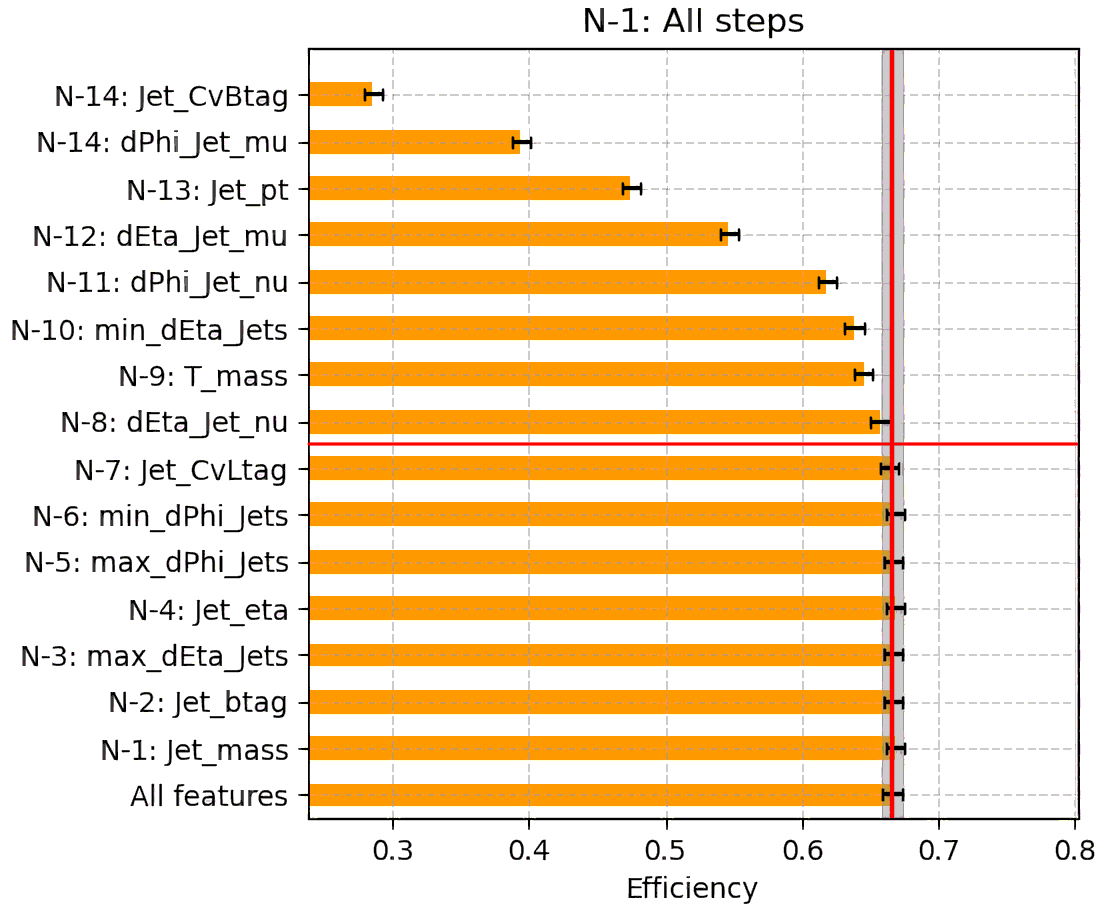
\includegraphics[width=1\linewidth]{fig//chap08-kin_reco/n_minus1.png}
        \caption{N-1 step. Highest ranking on the top.}
    \end{subfigure}
    \hfill
    \begin{subfigure}{0.9\linewidth}   
        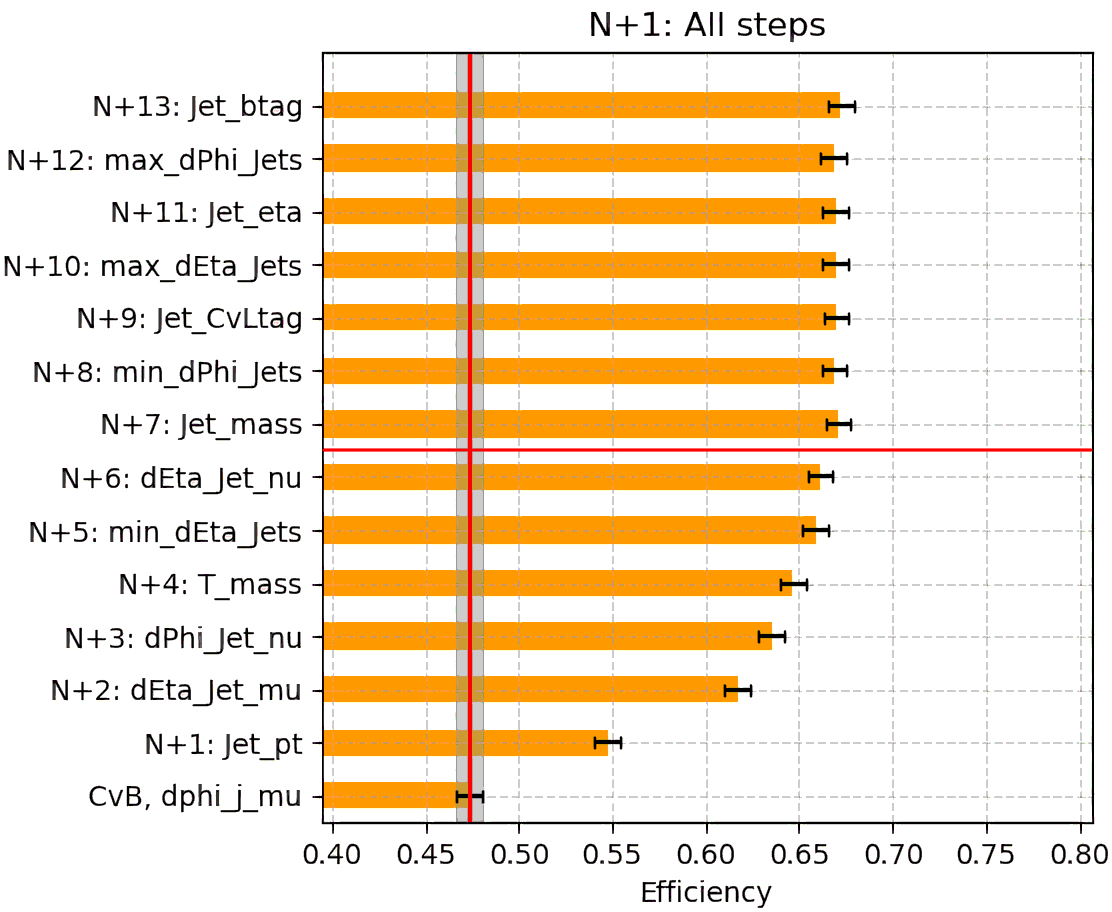
\includegraphics[width=1\linewidth]{fig//chap08-kin_reco/n_plus1.png}
        \caption{N+1 step. Highest ranking on the bottom.}
    \end{subfigure}  
    \caption{Jet-wise N+1,N-1 feature ranking.}
    \label{fig:n_rank}
\end{figure}




\begin{figure}[H]
    \vspace{-0.5cm}
    \centering
    \begin{subfigure}{0.513\linewidth}
        \centering
        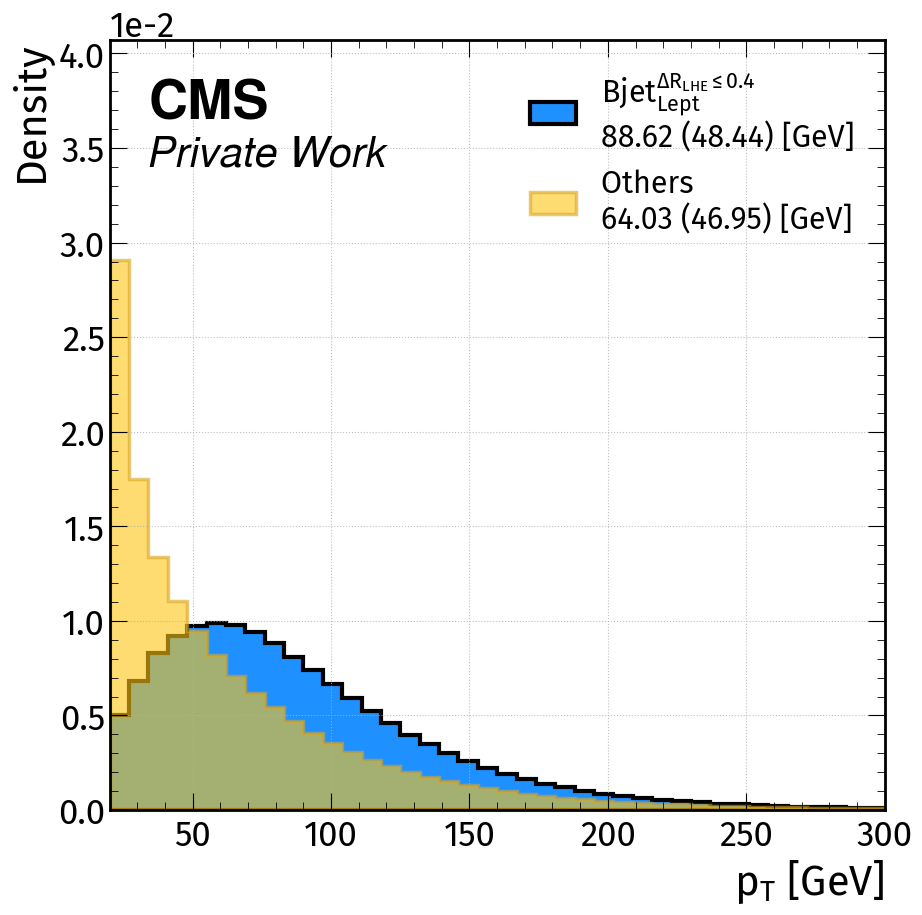
\includegraphics[width=1\linewidth]{fig//chap08-kin_reco/Jet_pt.png}
        \caption{Jet $p_T$}
    \end{subfigure}
    \hfill
    \begin{subfigure}{0.47\linewidth}  
        \centering
        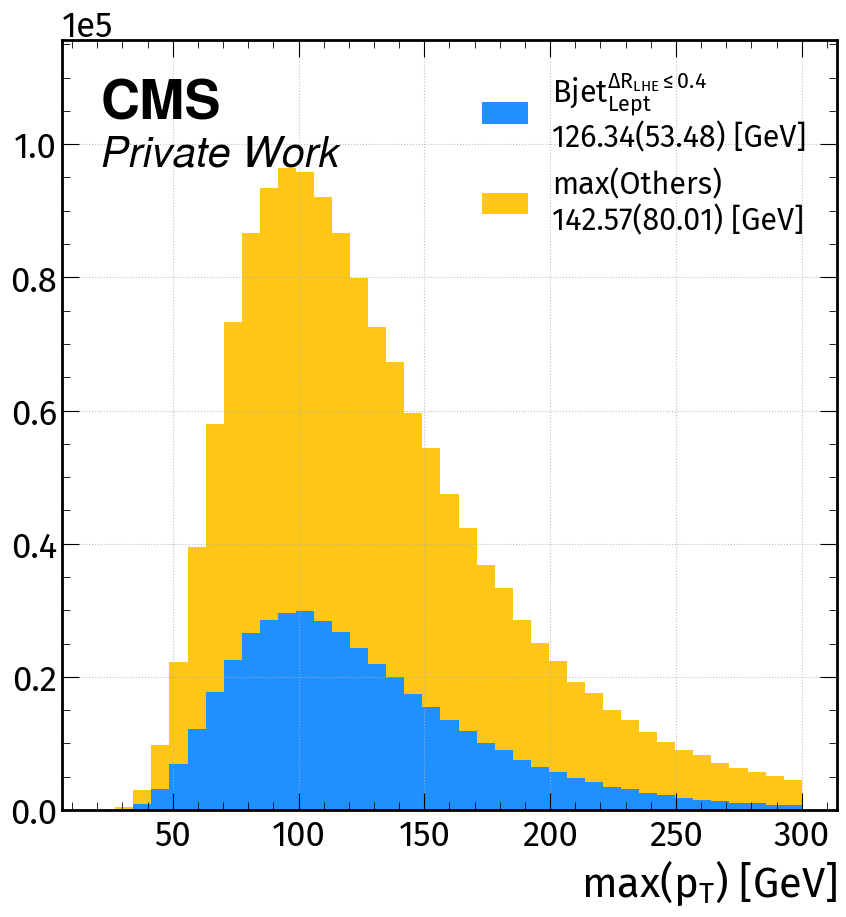
\includegraphics[width=1\linewidth]{fig//chap08-kin_reco/max_Pt.png}
        \caption{max Jet $p_T$}
    \end{subfigure}  
    \hfill
    \begin{subfigure}{0.513\linewidth}
        \centering
        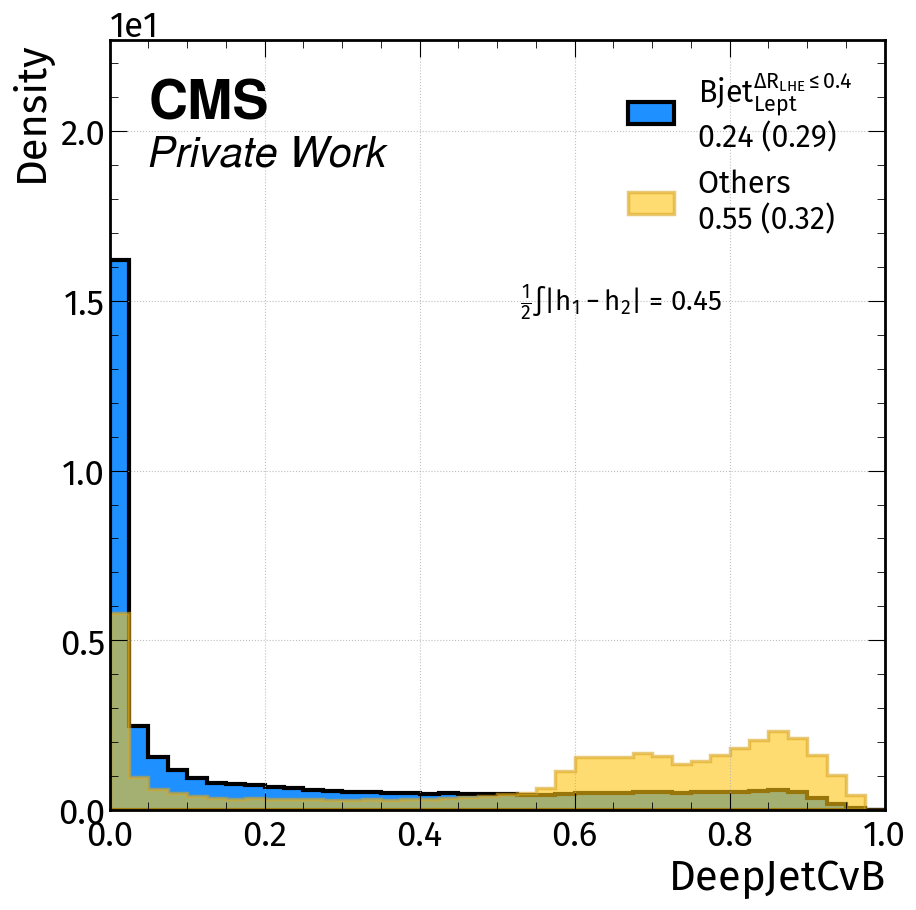
\includegraphics[width=1\linewidth]{fig//chap08-kin_reco/cvb.png}
        \caption{Jet\_CvB}
    \end{subfigure}
    \hfill
    \begin{subfigure}{0.47\linewidth}  
        \centering
        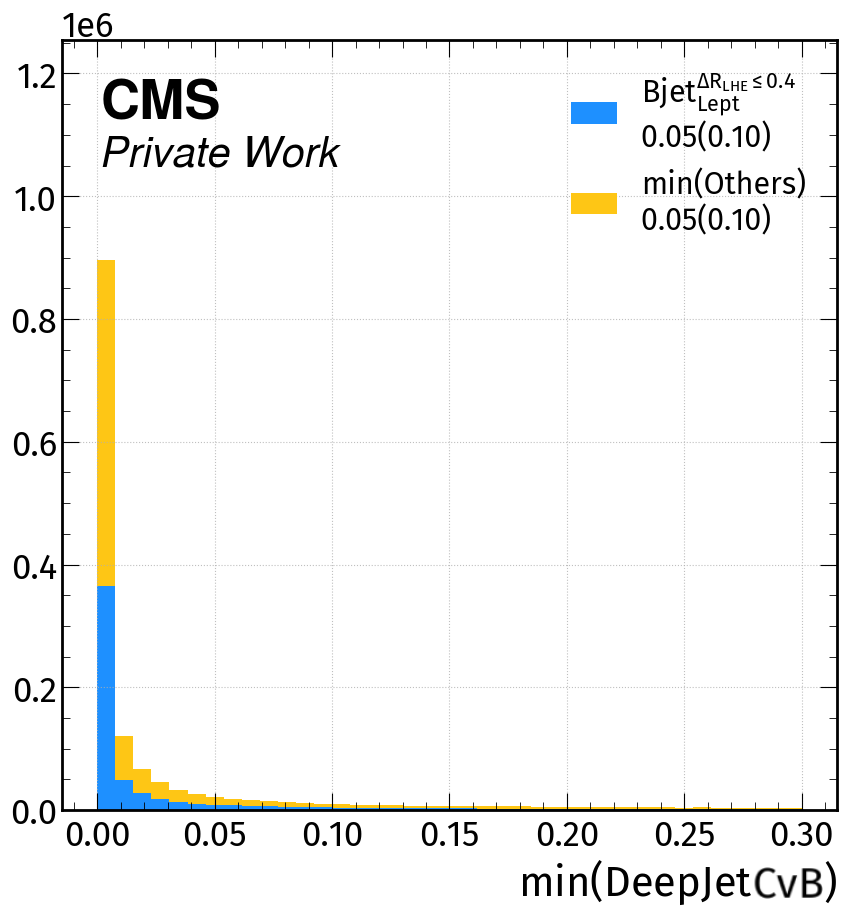
\includegraphics[width=1\linewidth]{fig//chap08-kin_reco/min_cvb.png}
        \caption{min Jet\_CvB}
    \end{subfigure} 
    \hfill
    \begin{subfigure}{0.513\linewidth}
        \centering
        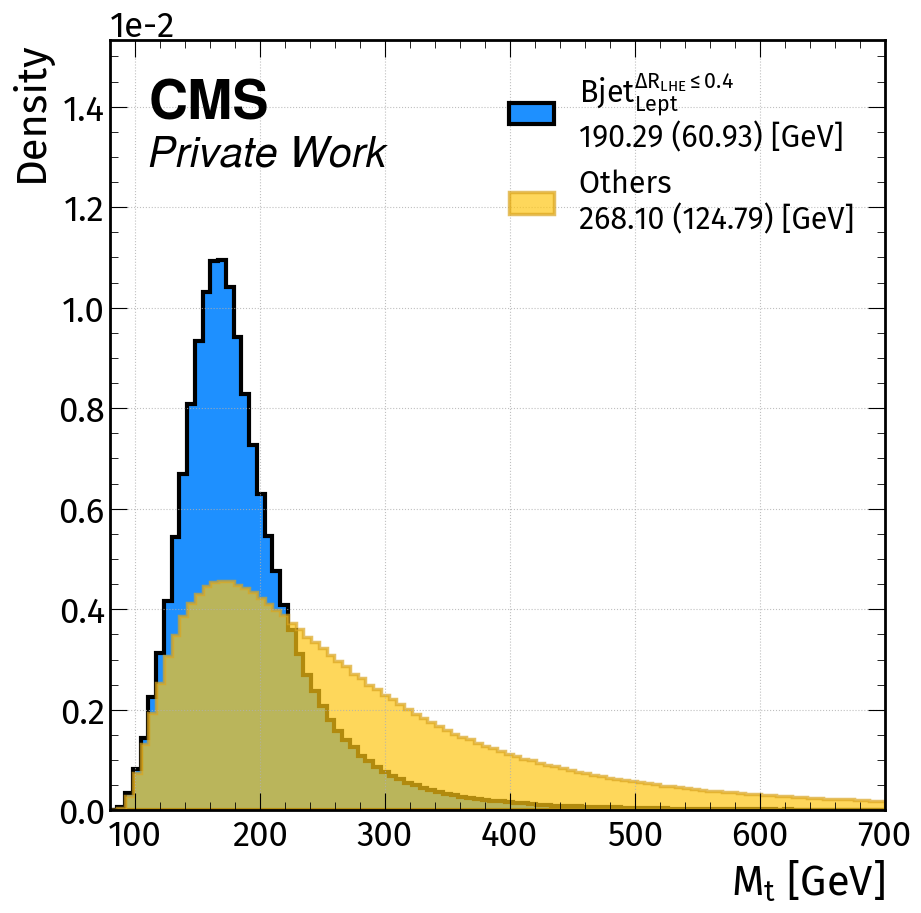
\includegraphics[width=1\linewidth]{fig//chap08-kin_reco/Tmass.png}
        \caption{$m_t$}
    \end{subfigure}
    \hfill
    \begin{subfigure}{0.47\linewidth}  
        \centering
        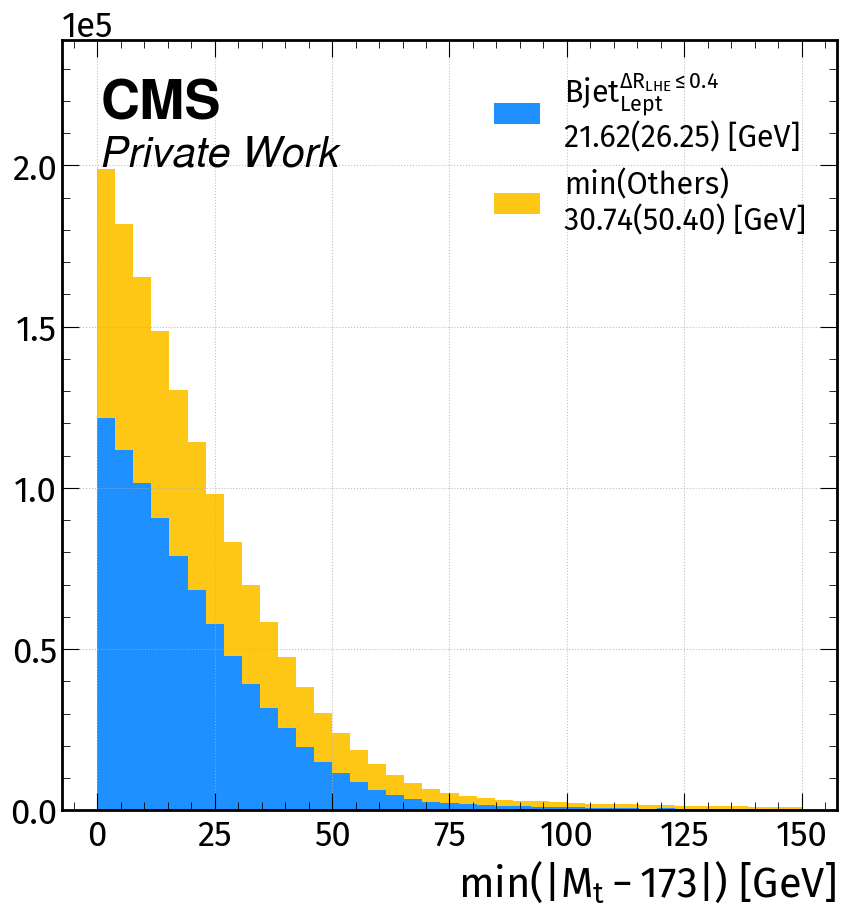
\includegraphics[width=1\linewidth]{fig//chap08-kin_reco/min_Tmass.png}
        \caption{$\min(|m_t-173|)$}
    \end{subfigure}  
\end{figure}





\begin{figure}[H]
    \ContinuedFloat
    \vspace{-0.5cm}
    \centering
    
     \begin{subfigure}{0.49\linewidth}
        \centering
        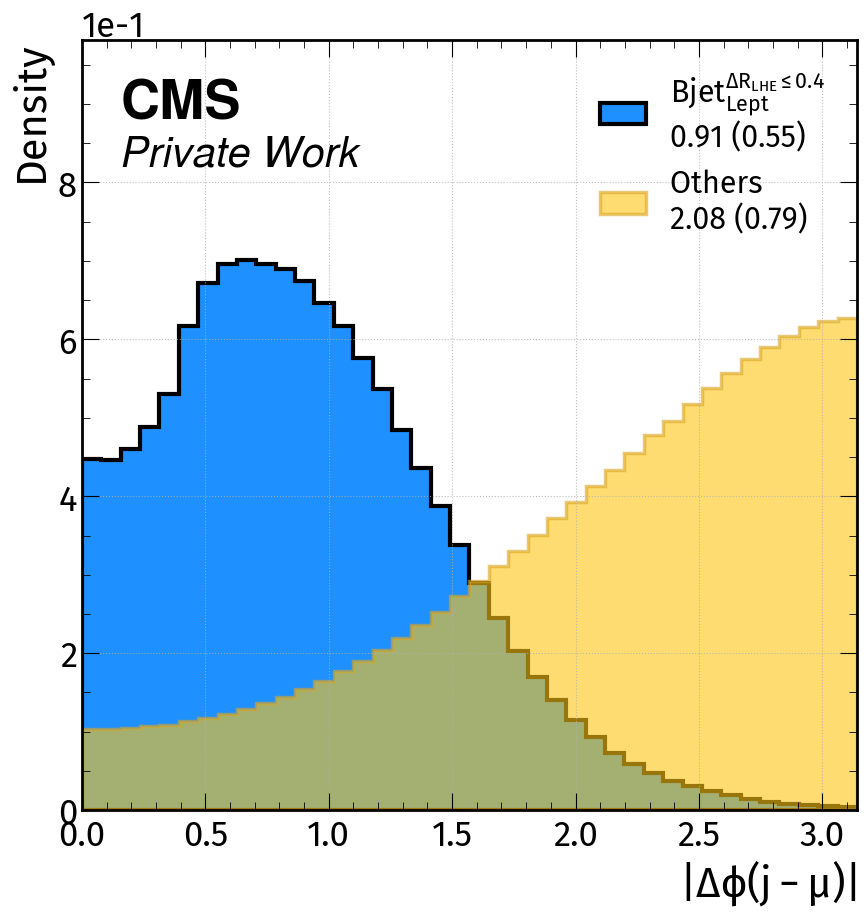
\includegraphics[width=1\linewidth]{fig//chap08-kin_reco/dphi_mu.png}
        \caption{$|\Delta \phi|$ Jet-$\mu$}
    \end{subfigure}
    \hfill
    \begin{subfigure}{0.46\linewidth}  
        \centering
        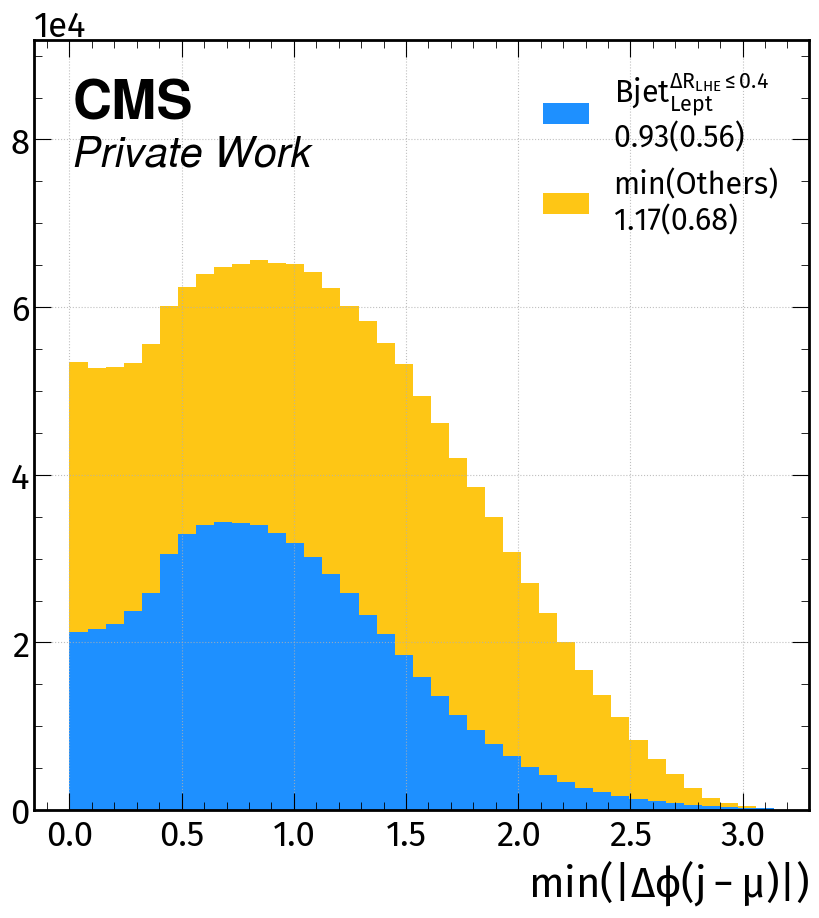
\includegraphics[width=1\linewidth]{fig//chap08-kin_reco/min_dphi_mu.png}
        \caption{$\min |\Delta \phi|$ Jet-$\mu$}
    \end{subfigure}  
    \hfill
    \begin{subfigure}{0.49\linewidth}
        \centering
        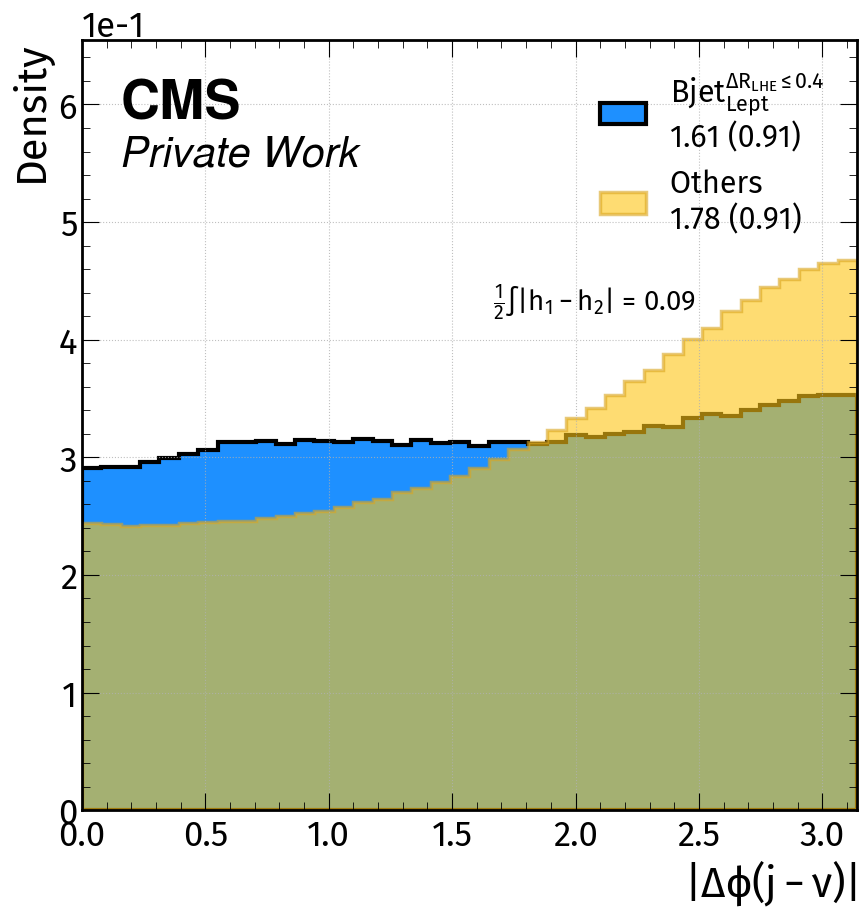
\includegraphics[width=1\linewidth]{fig//chap08-kin_reco/dphi_nu.png}
        \caption{$|\Delta \phi|$ Jet-$\nu$}
    \end{subfigure}
    \hfill
    \begin{subfigure}{0.48\linewidth}  
        \centering
        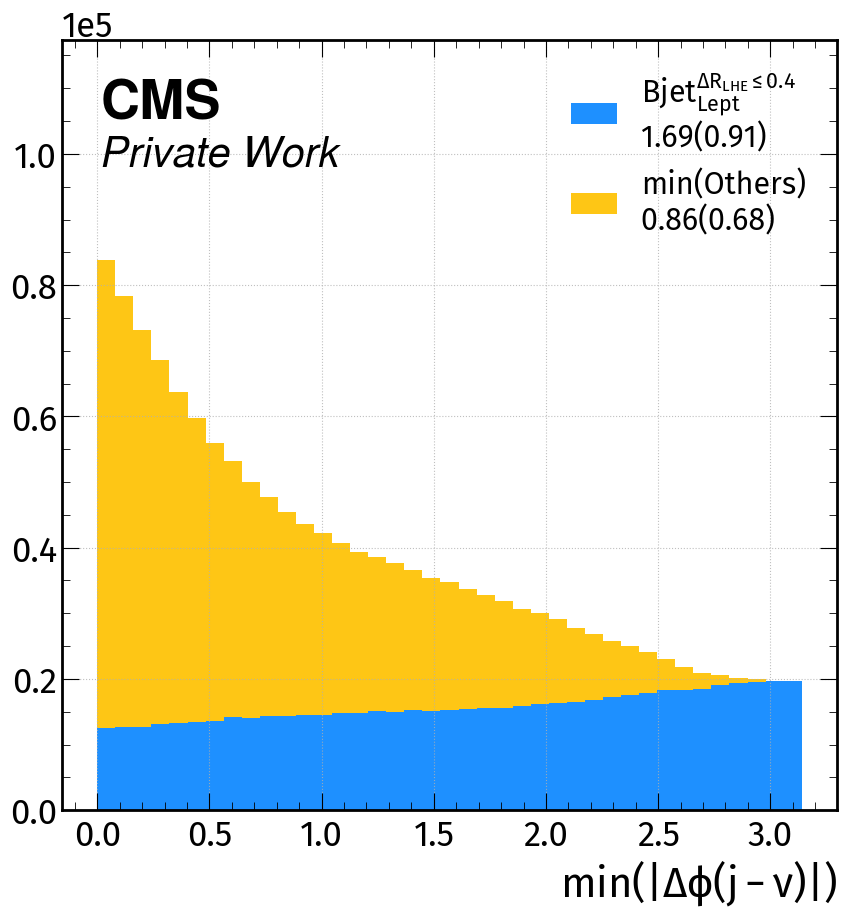
\includegraphics[width=1\linewidth]{fig//chap08-kin_reco/min_dphi_nu.png}
        \caption{$\min |\Delta \phi|$ Jet-$\nu$}
    \end{subfigure} 
    \hfill
    \begin{subfigure}{0.49\linewidth}
        \centering
        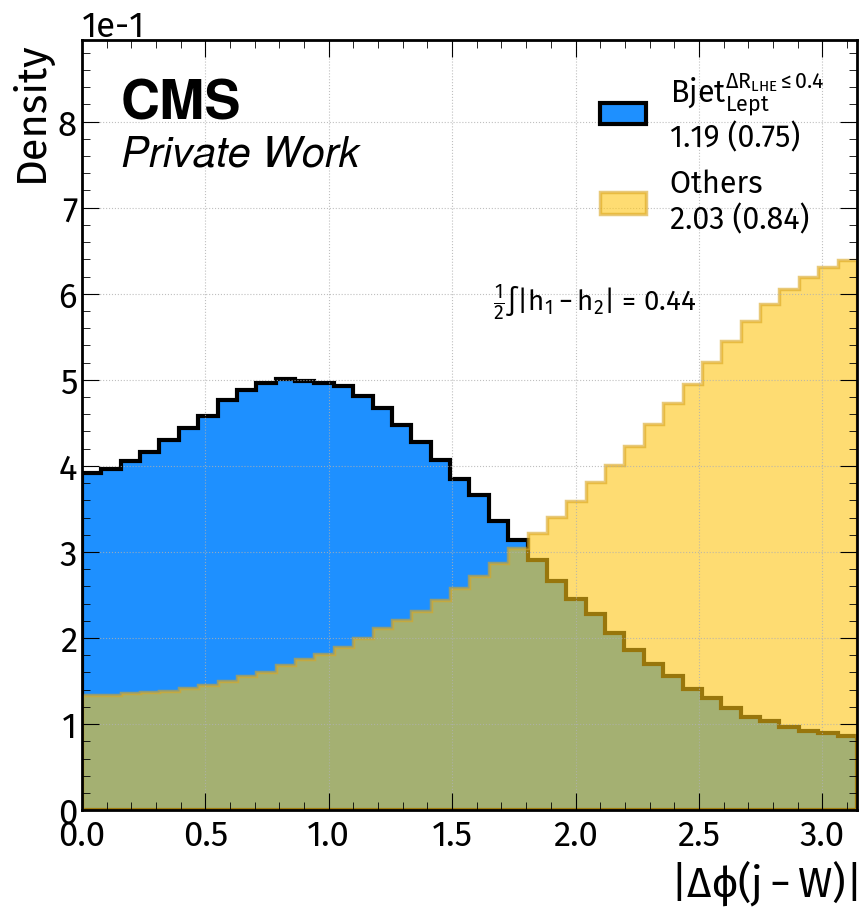
\includegraphics[width=1\linewidth]{fig//chap08-kin_reco/dphi_W.png}
        \caption{$|\Delta \phi|$ Jet-$\PW$}
    \end{subfigure}
    \hfill
    \begin{subfigure}{0.46\linewidth}  
        \centering
        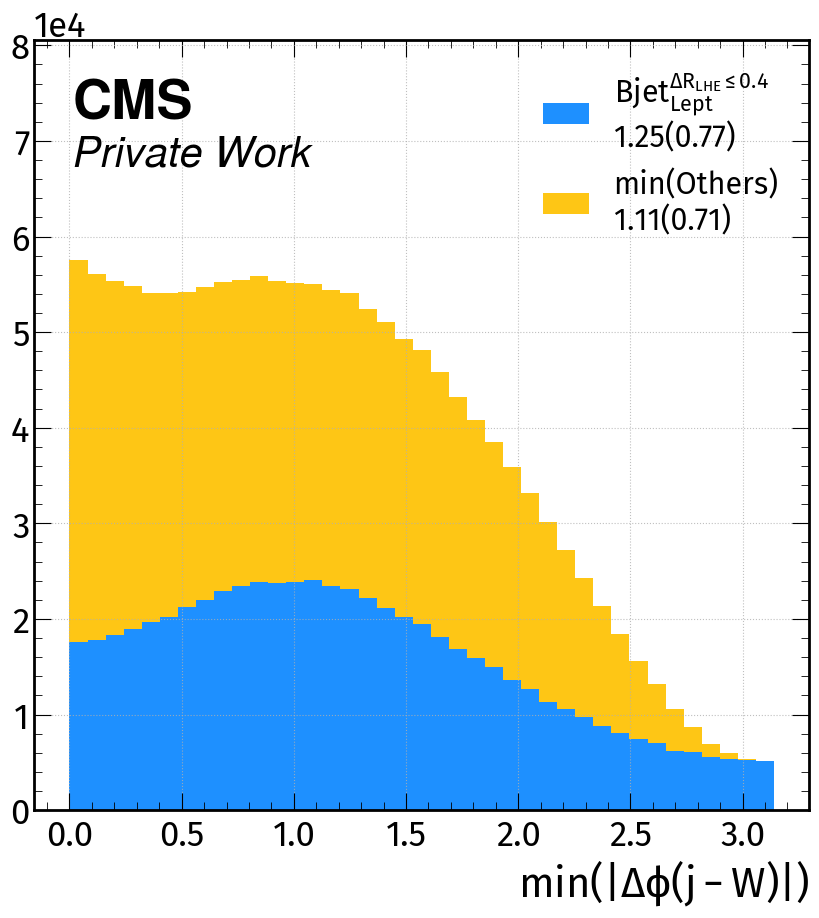
\includegraphics[width=1\linewidth]{fig//chap08-kin_reco/min_dphi_W.png}
        \caption{$\min|\Delta \phi|$ Jet-$\PW$}
    \end{subfigure}  
\end{figure}
\newpage
\begin{figure}[H]
    \ContinuedFloat
    \vspace{-0.5cm}
    \centering
     \begin{subfigure}{0.49\linewidth}
        \centering
        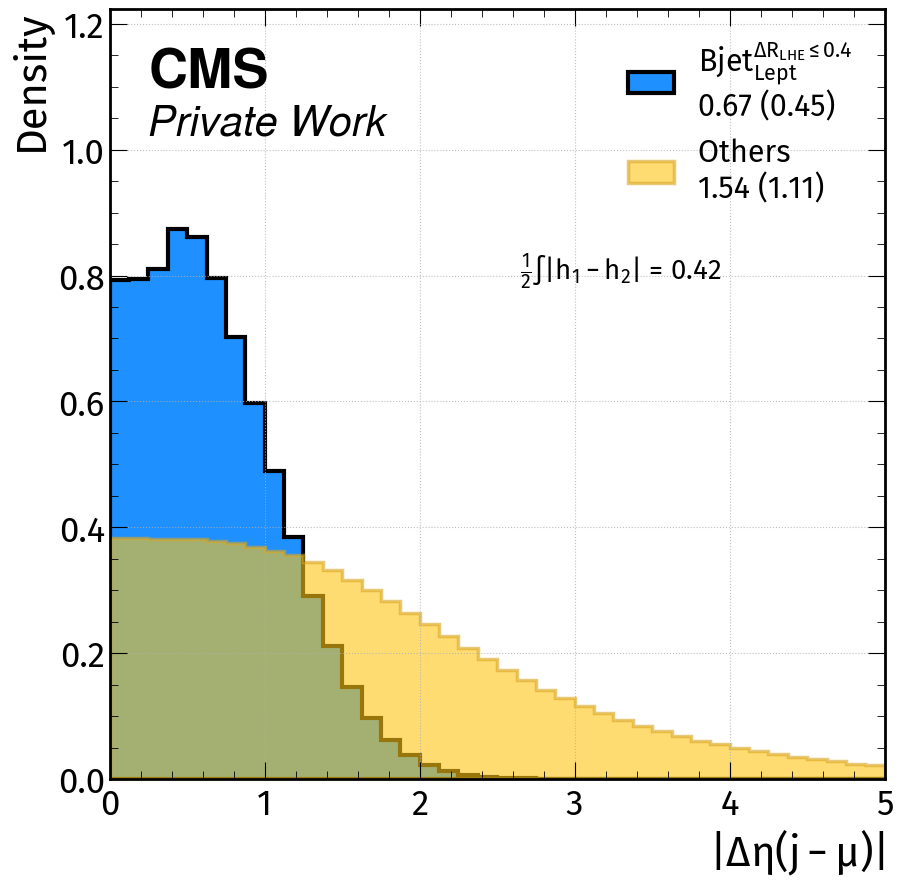
\includegraphics[width=1\linewidth]{fig//chap08-kin_reco/deta_mu.png}
        \caption{$|\Delta \eta|$ Jet-$\mu$}
    \end{subfigure}
    \hfill
    \begin{subfigure}{0.47\linewidth}  
        \centering
        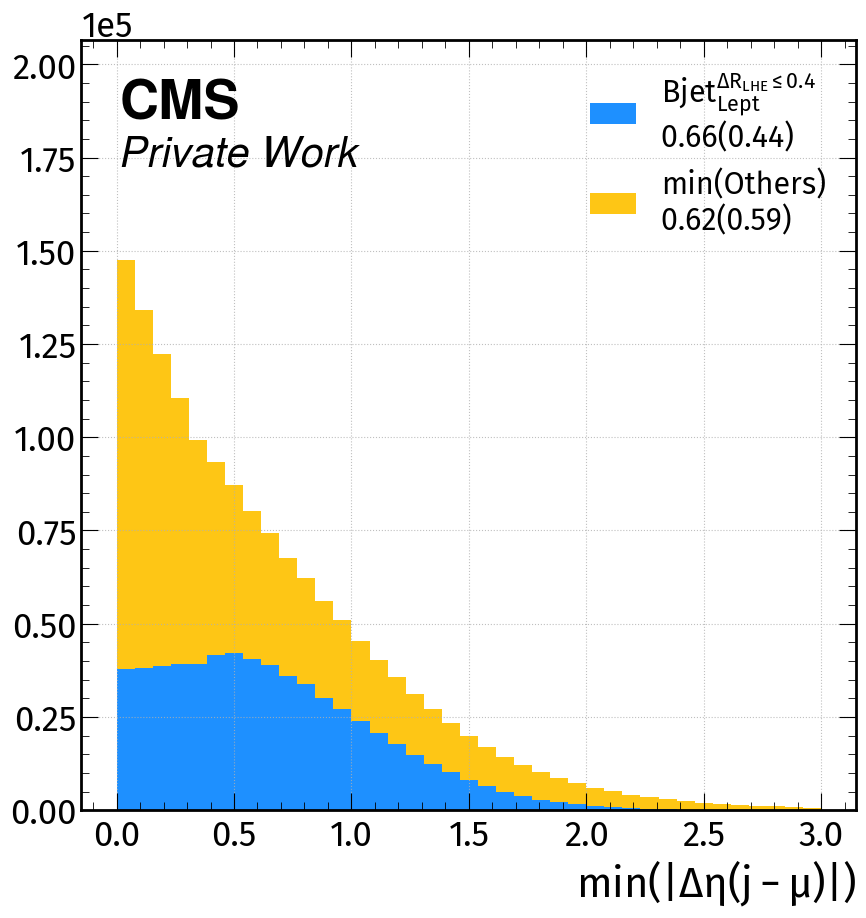
\includegraphics[width=1\linewidth]{fig//chap08-kin_reco/min_deta_mu.png}
        \caption{$\min|\Delta \eta|$ Jet-$\mu$}
    \end{subfigure}  
    \hfill
    \begin{subfigure}{0.49\linewidth}
        \centering
        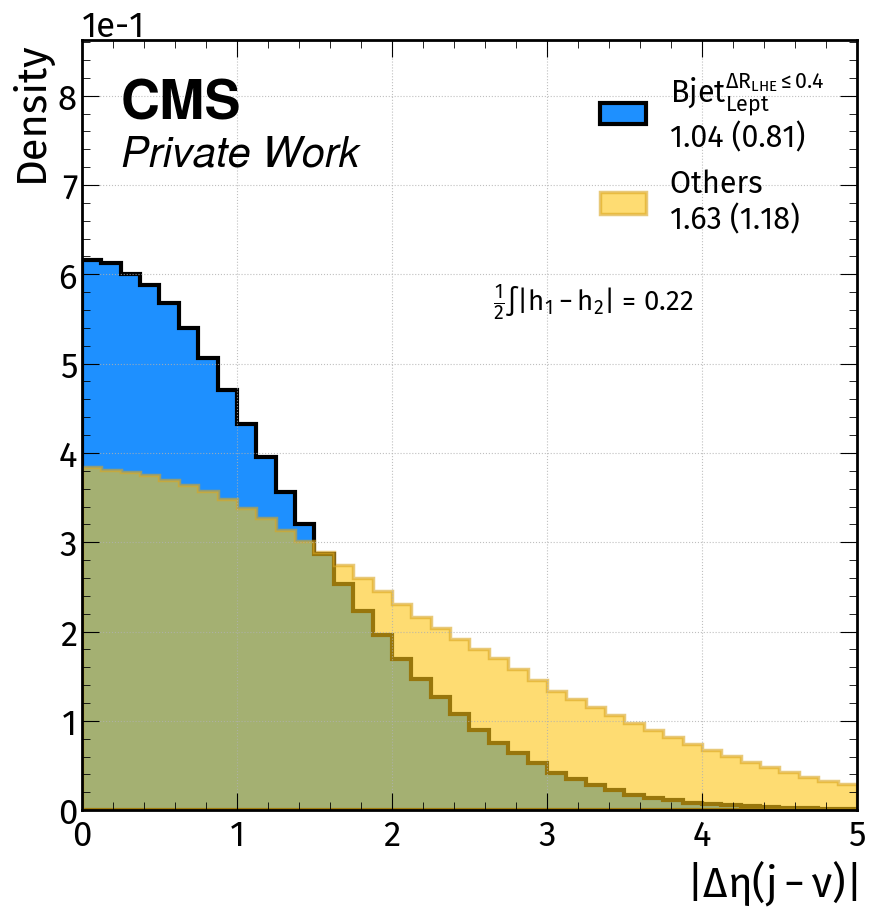
\includegraphics[width=1\linewidth]{fig//chap08-kin_reco/deta_nu.png}
        \caption{$|\Delta \eta|$ Jet-$\nu$}
    \end{subfigure}
    \hfill
    \begin{subfigure}{0.4825\linewidth}  
        \centering
        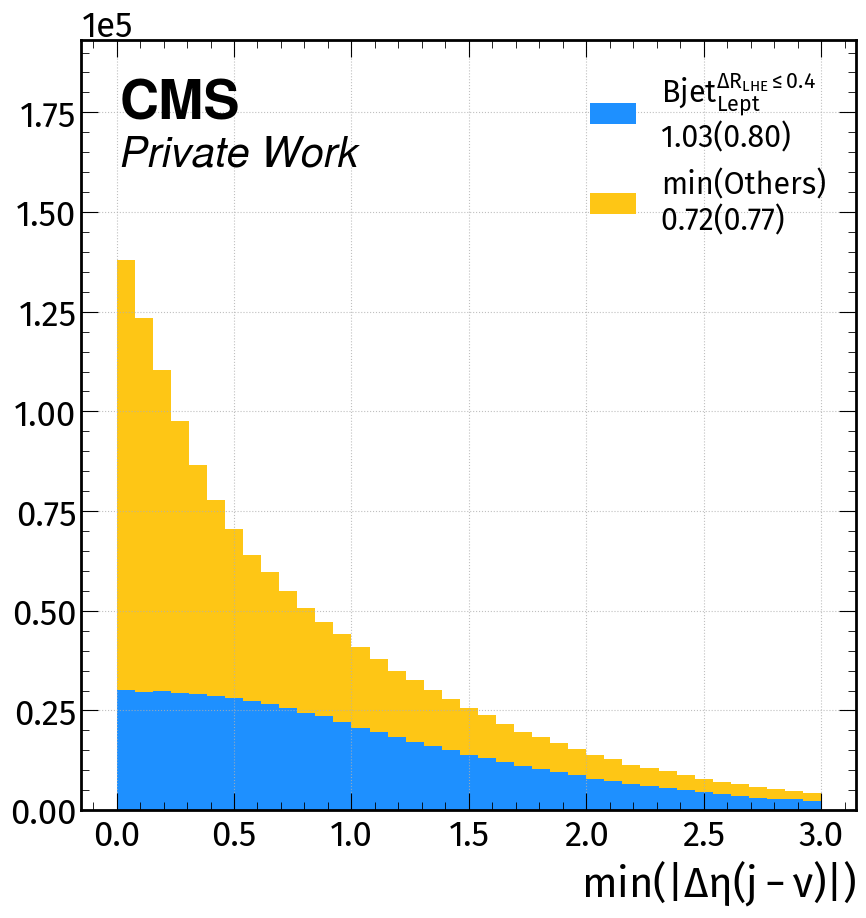
\includegraphics[width=1\linewidth]{fig//chap08-kin_reco/min_deta_nu.png}
        \caption{$\min|\Delta \eta|$ Jet-$\nu$}
    \end{subfigure}  
    \hfill
    \begin{subfigure}{0.49\linewidth}
        \centering
        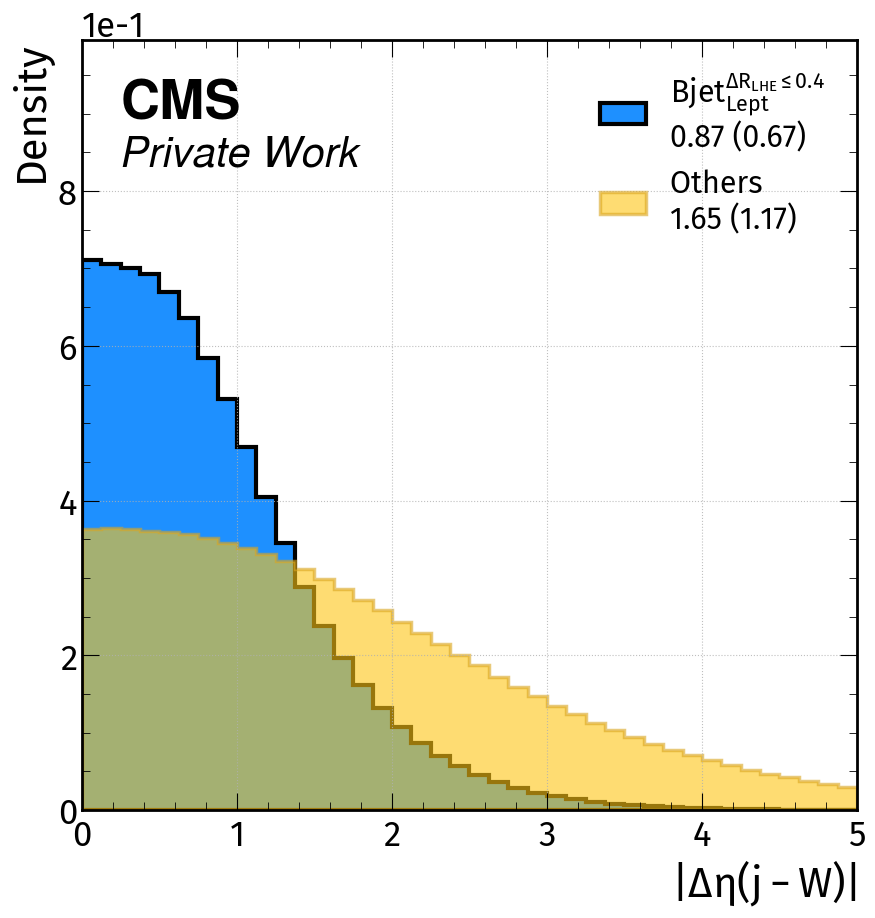
\includegraphics[width=1\linewidth]{fig//chap08-kin_reco/deta_W.png}
        \caption{$|\Delta \eta|$ Jet-$\PW$}
    \end{subfigure}
    \hfill
    \begin{subfigure}{0.4825\linewidth}  
        \centering
        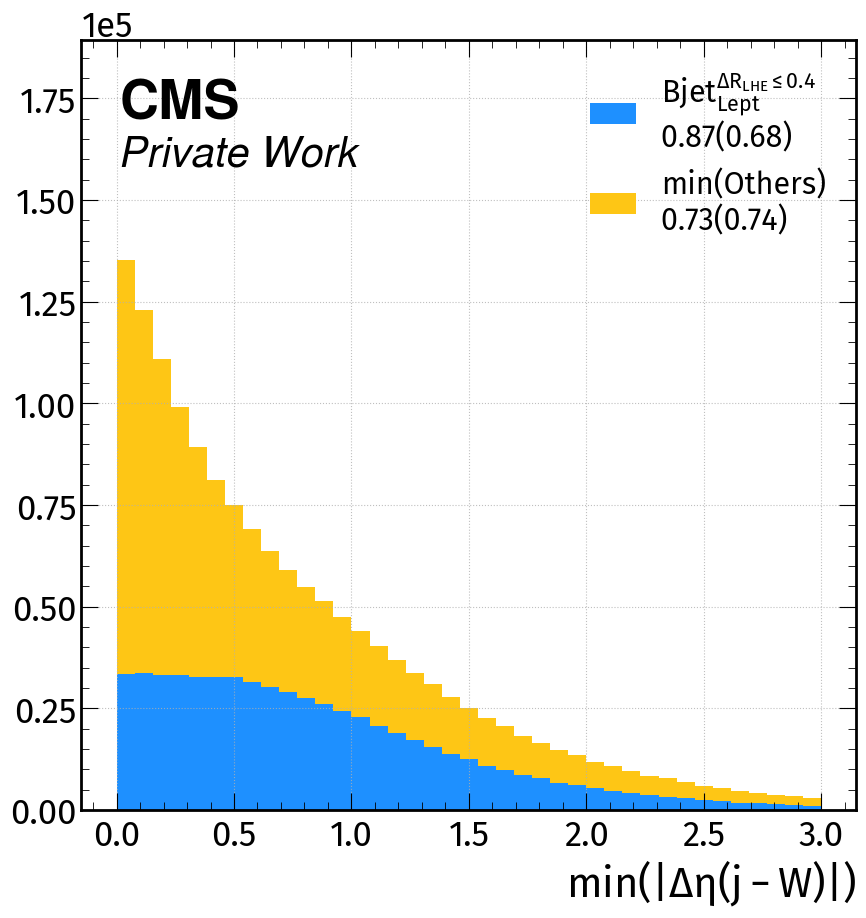
\includegraphics[width=1\linewidth]{fig//chap08-kin_reco/min_deta_W.png}
        \caption{$\min|\Delta \eta|$ Jet-$\PW$}
    \end{subfigure}  
\end{figure}
\newpage
\begin{figure}[H]
    \ContinuedFloat
    \vspace{-0.5cm}
    \centering
    \begin{subfigure}{0.49\linewidth}
        \centering
        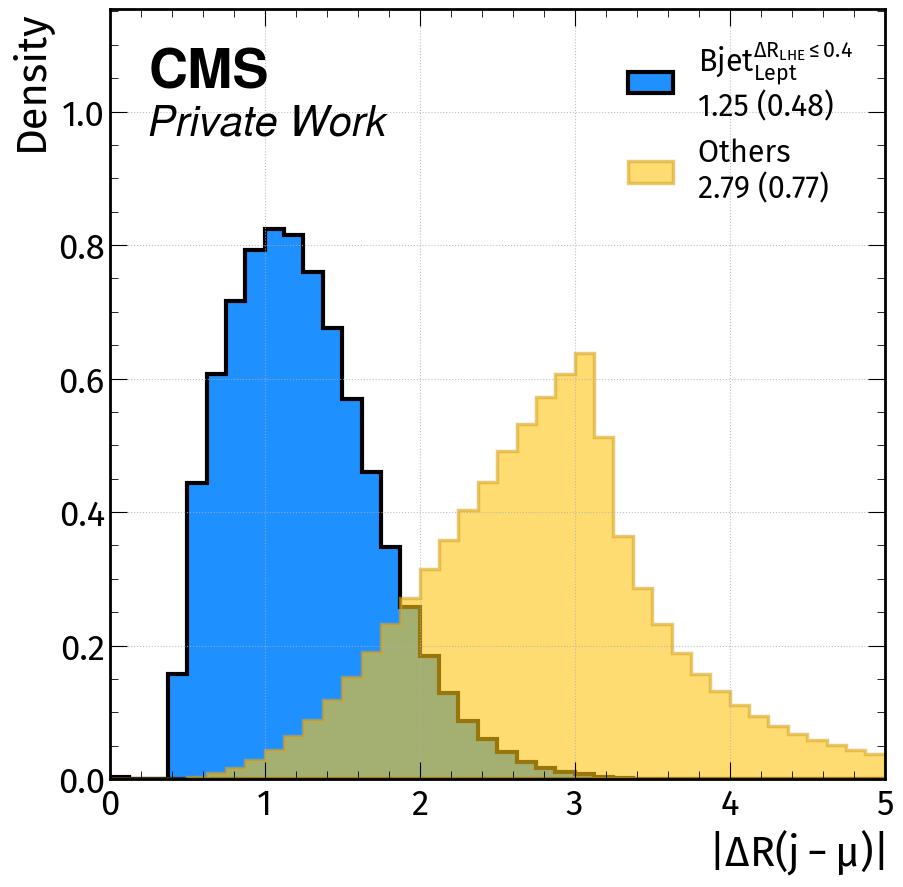
\includegraphics[width=1\linewidth]{fig//chap08-kin_reco/dr_mu.png}
        \caption{$\Delta R$ Jet-$\mu$}
    \end{subfigure}
    \hfill
    \begin{subfigure}{0.4585\linewidth}  
        \centering
        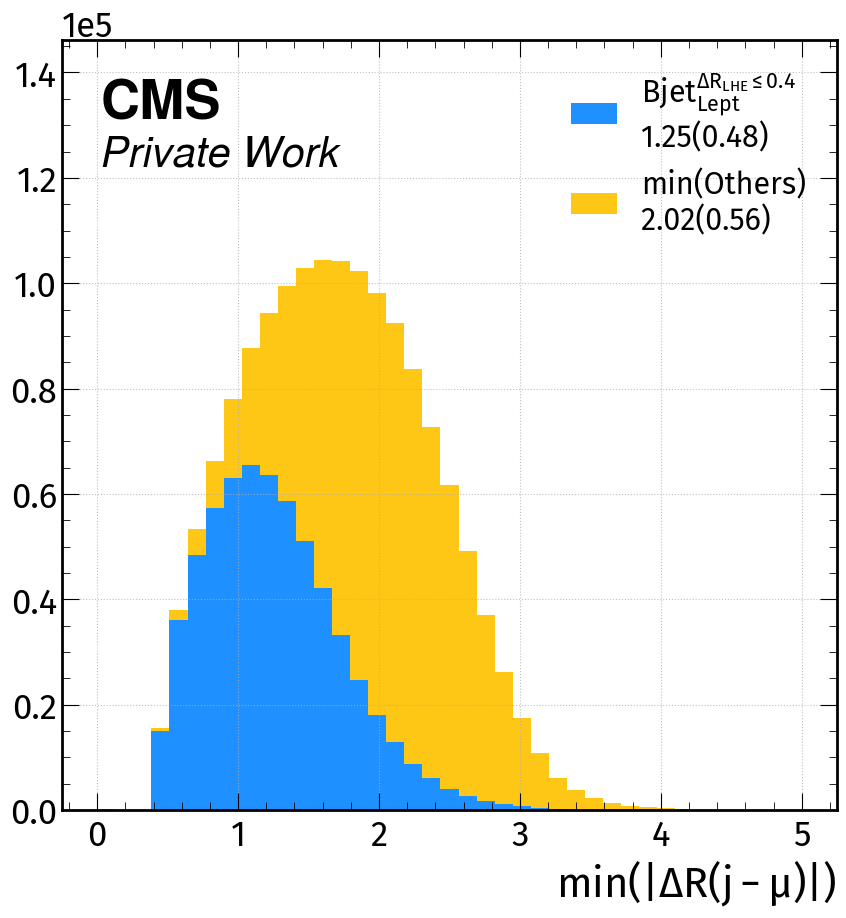
\includegraphics[width=1\linewidth]{fig//chap08-kin_reco/min_dr_mu.png}
        \caption{$\min \Delta R$ Jet-$\mu$}
    \end{subfigure}  
    \hfill
    \begin{subfigure}{0.49\linewidth}
        \centering
        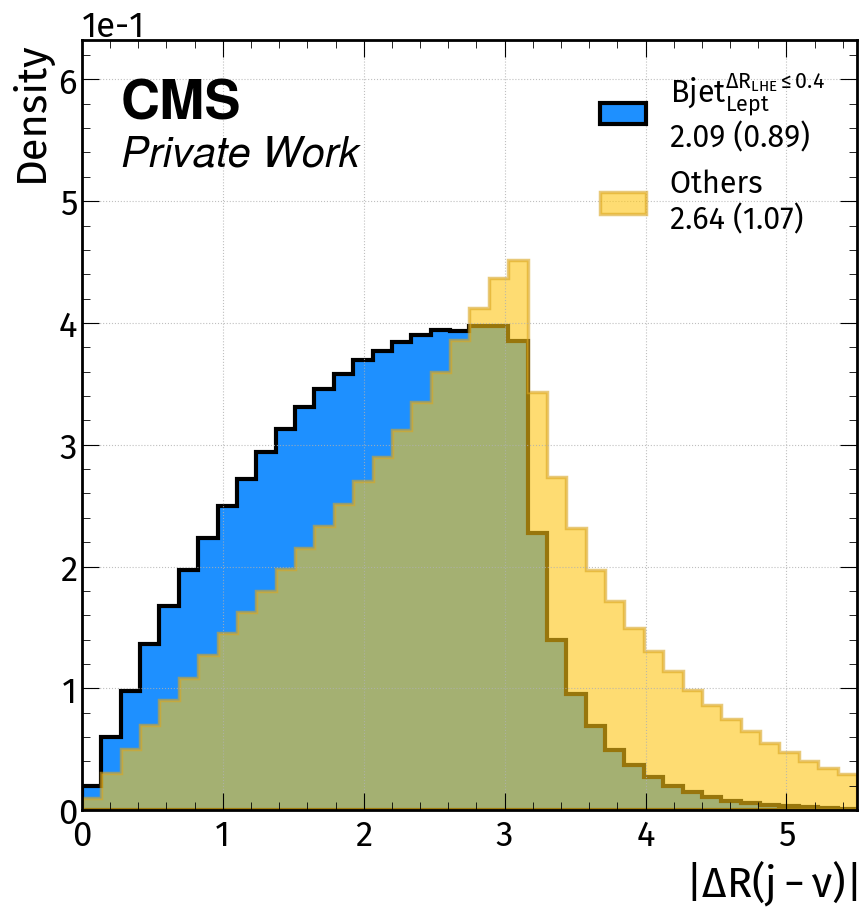
\includegraphics[width=1\linewidth]{fig//chap08-kin_reco/dr_nu.png}
        \caption{$\Delta R$ Jet-$\nu$}
    \end{subfigure}
    \hfill
    \begin{subfigure}{0.4775\linewidth}  
        \centering
        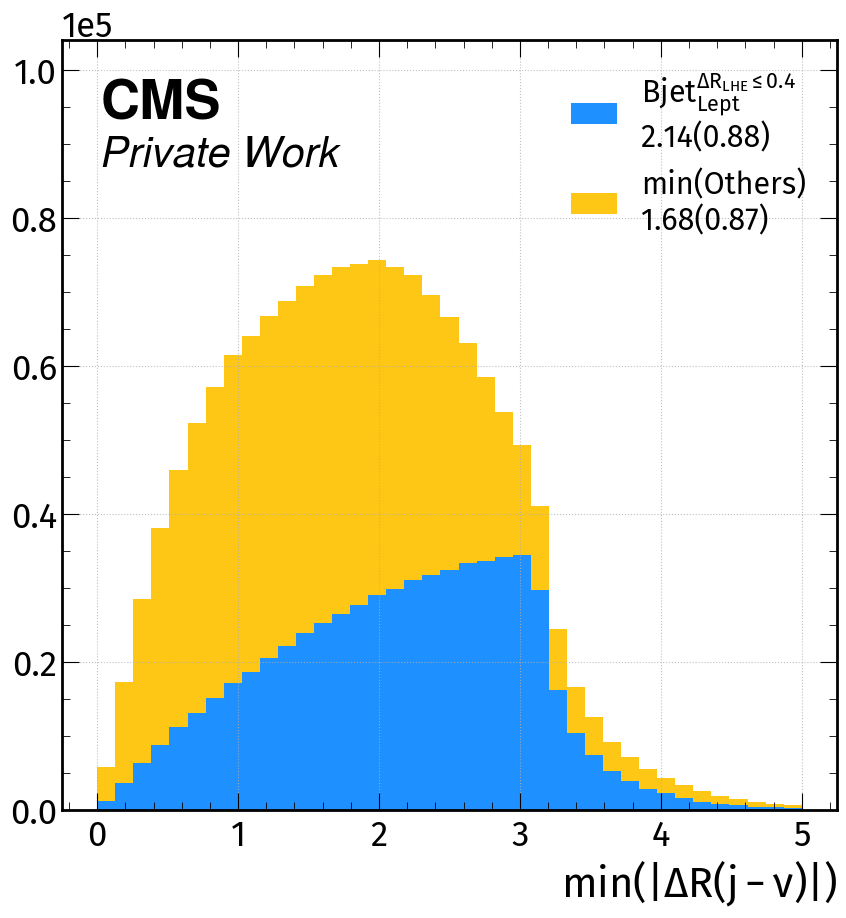
\includegraphics[width=1\linewidth]{fig//chap08-kin_reco/min_dr_nu.png}
        \caption{$\min \Delta R$ Jet-$\nu$}
    \end{subfigure}  
    \hfill
    \begin{subfigure}{0.49\linewidth}
        \centering
        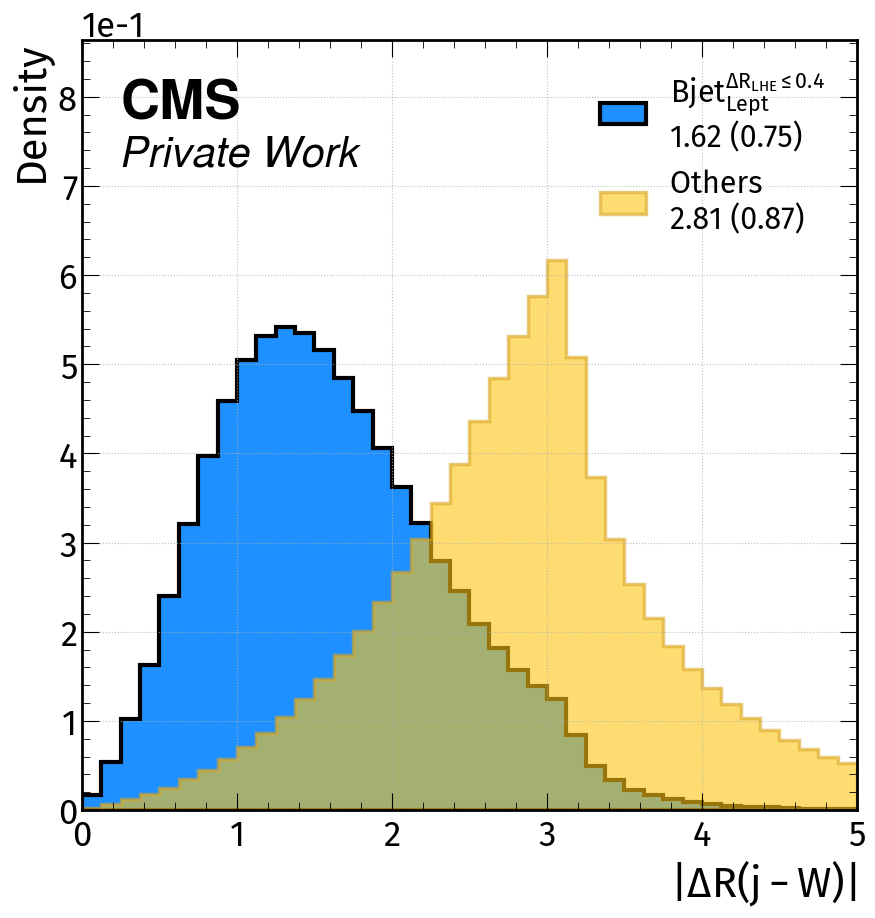
\includegraphics[width=1\linewidth]{fig//chap08-kin_reco/dr_W.png}
        \caption{$\Delta R$ Jet-$\PW$}
    \end{subfigure}
    \hfill
    \begin{subfigure}{0.475\linewidth}  
        \centering
        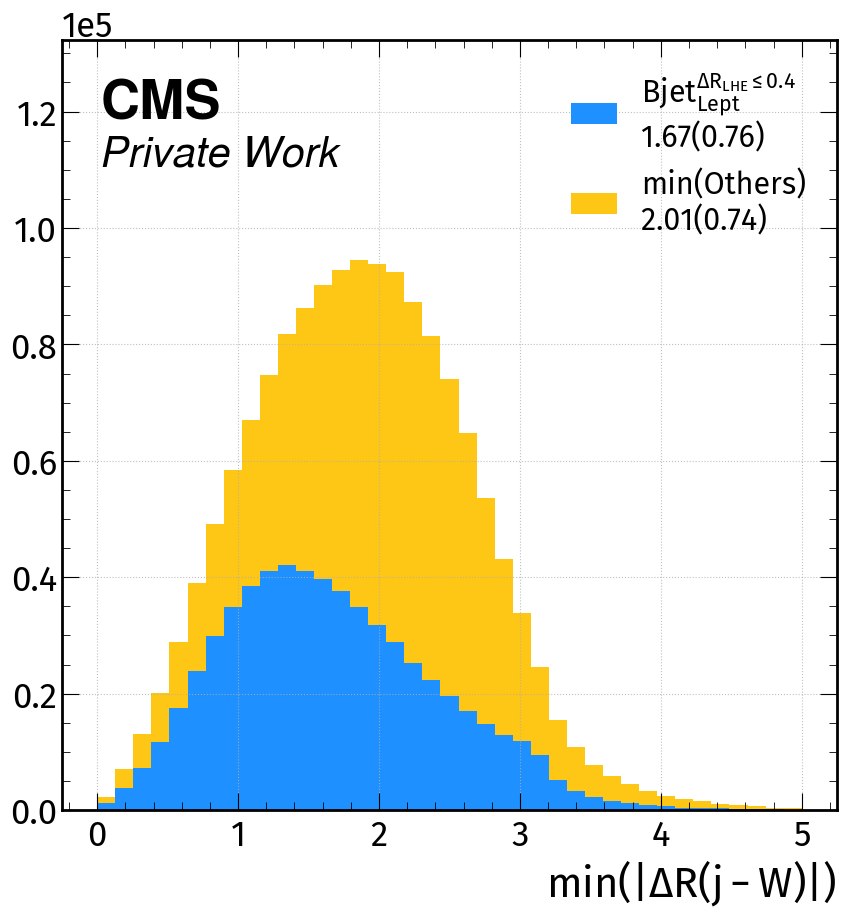
\includegraphics[width=1\linewidth]{fig//chap08-kin_reco/min_dr_W.png}
        \caption{$\min \Delta R$ Jet-$\PW$}
    \end{subfigure}  
\end{figure}

\newpage
\begin{figure}[H]
    \ContinuedFloat
    \vspace{-0.5cm}
    \centering
    \caption{Distibutions of the most relevant features. On the left side, there are the distributions of the observables of the leptonic b Jet and of the other jets, both normalized to 1.
On the right side, there are the stacked histograms of the distributions of the minimum or the maximum of each observable for each event.
The legend includes information on the mean and standard deviation.}
\end{figure}

\subsubsection*{Event-wise models}
Another category of models under examination falls into the event-wise models class. These models receive a matrix as input, where rows represent various events, and columns encompass diverse event and object characteristics. 
Event-wise models retain the event structure, providing a more direct approach to addressing the JPA problem and eliminating the need to reconstruct the event after the network evaluation.\\
\\
However, constructing such a model is not trivial: An MLP, for instance, would have a distinct set of input units for each jet or lepton, each assigned to different features, and N outputs, where N is the maximum number of jets in the events. The prediction would involve identifying the index of the predicted leptonic b Jet for each event.\\
\\
This approach has multiple criticalities:
\begin{itemize}
    \item Since the labels correspond to the index of the jet within the event, the model lacks permutation invariance, which necessitates introducing an order among the jets in the event.
    \item Although the network's output may appear as a straightforward index,  it constitutes a classification problem with N classes that leads to two complexities:
    \begin{itemize}
        \item[\ding{111}] The high dimensionality of the output space demands a significant amount of data for effective population, a well-known challenge referred to as the "curse of dimensionality."
        \item[\ding{111}] To address the imbalance between the N classes, the cross-entropy loss must be reweighted, but, since the network is not permutation invariant, neither is the reweighting.
    \end{itemize}
    \item N is the maximum number of jets considered in the event, but, when an event has less than M jets, dealing with the units related to the remaining N-M jets becomes a concern.\\
    We could discuss different methods to assign a value for the features of the absent jets, but no choice would be optimal.
\end{itemize}
To tackle these challenges, one potential solution involves leveraging an architecture better suited to the problem, such as attention networks. In the following section, we introduce a neural network based on the attention mechanism to address the JPA problem, which we will henceforth refer to as "JPANet" (Jet-Parton Attention Net) that afterward will be employed to tackle the full JPA problem.

\subsection{Full Jet-parton assignment}
\paragraph*{JPANet}
JPANet is an attention network adapted to the topology of the signal events.\\
The network takes in two different inputs: one representing the leptonic W boson, and the other containing the features of all the jets.\\
These inputs are channeled into separate subnetworks referred to as "heads" and are subsequently merged through a cross-attention mechanism.\\



\begin{minipage}{0.625\linewidth}
\begin{itemize}
    \item \textbf{W head}: The input tensor for the W head has a dimension of $(N_{\text{events}},1,7)$, with 7 representing the number of features related to the leading lepton and the reconstructed neutrino originating in the leptonic W decay listed in \Tab{tab:Whead}.\\
    The inputs are normalized with a Batch norm layer before being passed through a feed-forward network consisting of two layers, each containing 80 units.
    The resulting output from the W head constitutes the "W embedding."
\end{itemize}
\end{minipage}
    \hfill
\begin{minipage}{0.33\linewidth}
        \centering
        \fontsize{11pt}{11pt}\selectfont
        \begin{tabular}{c|c}
            \toprule
             \textbf{Feature}& \textbf{Description} \\
             \midrule
             
             $p_T^\ell$& Lepton $p_T$ \\
             $\phi^\ell$& Lepton $\phi$ \\
             $\eta^\ell$& Lepton $\eta$ \\
             \midrule
             $ p_T^\nu$& Neutrino $p_T$ \\
             $\phi^\nu$& Neutrino $\phi$ \\
             $\eta^\nu$& Neutrino $\eta$ \\
             \midrule
             \multirow{2}{*}{$m_W$} &Leptonic W\\
             &mass\\
             \bottomrule
        \end{tabular}
        \label{tab:Whead}
        \captionof{table}{W head features.}
\end{minipage}
\\
\begin{itemize}

\begin{minipage}{0.6\linewidth}
    \item \textbf{Jet head}: The input tensor for the Jet head has dimensions of  $(N_{\text{events}},7,5)$, where the second dimension corresponds to the various jets and the third dimension pertains to distinct features.\\
    These input features encompass the kinematic properties of each jet, alongside its CvB score and the invariant mass of the combined jet-lepton-neutrino system.\\
\end{minipage}
\hfill
\begin{minipage}{0.35\linewidth}
        \centering
        \fontsize{11pt}{11pt}\selectfont
        \begin{tabular}{c|c}
            \toprule
             \textbf{Feature}& \textbf{Description} \\
             \midrule               
             $p_T^j$& Jet $p_T$ \\
             $\phi^j$& Jet $\phi$ \\
             $\eta^j$& Jet $\eta$ \\
             $ m_{t_L}$& Lept. top mass \\
             Jet\_CvB& \DeepJet CvB\\
             \bottomrule
        \end{tabular}
        \captionof{table}{Jet head features.}
\end{minipage}
    Because in approximately 97\% of events, all the jets matching the four quark partons can be found among the $p_T$ leading seven jets with the highest transverse momentum, we opted to limit our selection to just seven jets (\Fig{fig:jets_stack}).\\
    These selected inputs are first passed through a batch normalization layer\footnote{Since $m_{t_L}$ can have significant outliers, the variable is first transformed with the function $\log(1+m_{t_L})$} and then through a feed-forward neural network, which consists of two layers, each containing 80 units.
    The output from the first MLP serves as the input for a residual network, comprising a self-attention layer and a layer normalization layer. Finally, the output from the self-attention jet ResNet is directed into another MLP, which consists of three layers, each having 80 units. The output of the jet head constitutes the "Jet embedding."
\end{itemize}


After creating the W and the Jet embedding, we exploit a cross-attention layer to combine all the information of the events to assign an attention score to each jet in the jet sequence. This process involves concatenating the W embedding and jet embedding sequences and employing them as the Key and Value components in the scaled dot product, with the Query derived from the jet embedding sequence.

\begin{minipage}{0.33\linewidth}
\vspace{-1cm}
\begin{figure}[H]
    \raggedright
    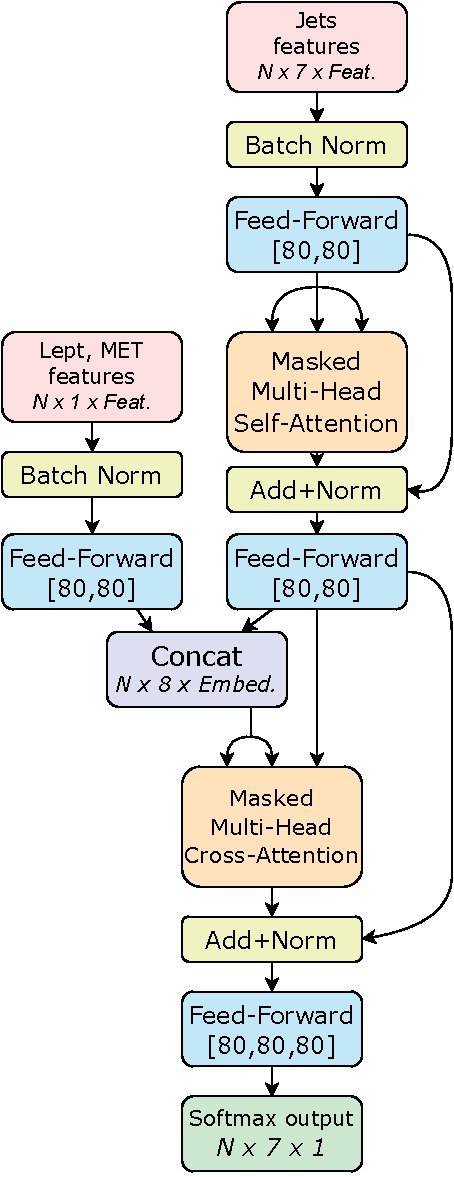
\includegraphics[width=\linewidth]{fig//chap08-kin_reco/JPANet_1.pdf}
    \caption{JPANet.}
    \label{fig:JPANet1}
\end{figure}
\end{minipage}
\hfill
\begin{minipage}{0.62\linewidth}
\vspace{-0.3cm}
The output of the cross-attention layer is added to the jet embedding residuals, normalized, and subsequently passed into the final Multi-Layer Perceptron (MLP), which consists of three layers, each containing 80 units. The output layer is equipped with a softmax function, ensuring that the outputs represent scores for each element in the jet sequence that are normalized to sum up to 1.\\
\\
The network employs the Swish activation function and includes a 1.2\% dropout probability to mitigate overfitting. Additionally, it utilizes a batch size of 20,000 and the RAdam optimizer, which minimizes the cross-entropy loss with a learning rate of $10^{-3}$.\\
Since the networks took 3 hours to train on an Nvidia A100 (40GB) GPU shared with the entire CERN community, a comprehensive hyperparameter optimization strategy could not be implemented. As a result, the choices made are based on a small number of trial runs.\\
Thanks to its architecture, JPA effectively addresses all the issues that an event-wise MLP would encounter. The network inherently maintains permutation invariance for physics objects and the absent jets are handled just by forcing their respective attention scores to zero.
\end{minipage}


\paragraph*{Leptonic bJet Performace} On both the training and validation datasets, JPANet successfully matched the correct jet to the leptonic b quark parton in 82\% of the events. This high accuracy represents a substantial enhancement compared to all the assessed jet-wise models, making JPANet the preferred choice for carrying out the complete JPA task.




\paragraph*{Full Jet-parton assignment}
To carry out the full JPA task using JPANet, a modification is needed primarily in the output layer. The chosen approach involves generating an output, denoted as $A_{jp}$,  for each event, with a shape of (7, 4), such that $\sum_j A_{jp}=1 \: \forall p$.
In other words, to each quark parton, are assigned one score per jet that sum up to one.
Additionally, since now we are looking for jets of different flavors, the \DeepJet CvL score is introduced in the jet features.
The optimal combination of jets is determined by maximizing the product of scores across all possible combinations of assigning the jets to the four quark partons.
Despite a significant number of potential combinations ($7!/(7-4)!=840$ in total), JPANet demonstrated the ability to accurately identify the correct jet-parton assignments in 54\% of the events in both the training and validation datasets.

\vspace{-0.2cm}
\begin{table}[H]
    \centering
    \fontsize{10.pt}{10.pt}\selectfont
    \begin{tabular}{l|c}
    \toprule
    \multicolumn{2}{c}{\textbf{JPANet accuracy}}\\
    \midrule
         \textbf{Lept. b JPA}& 82\%\\
         \textbf{Full JPA}& 54\%\\
    \end{tabular}
\end{table}




\begin{figure}[H]
    \vspace{-0.5cm}
    \centering
     \begin{subfigure}{0.434\linewidth}
        \centering
        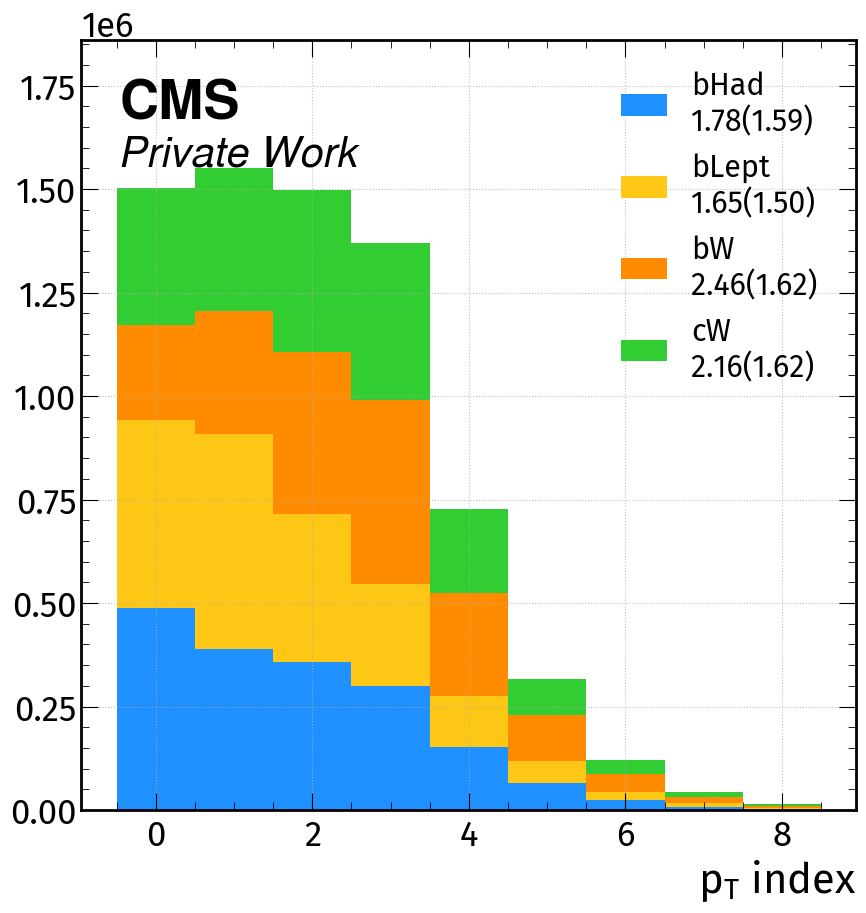
\includegraphics[width=1\linewidth]{fig//chap08-kin_reco/jets/pt_index.png}
        \caption{Jets $p_T$ index}
    \end{subfigure}
    \hfill
    \begin{subfigure}{0.4227\linewidth}  
        \centering
        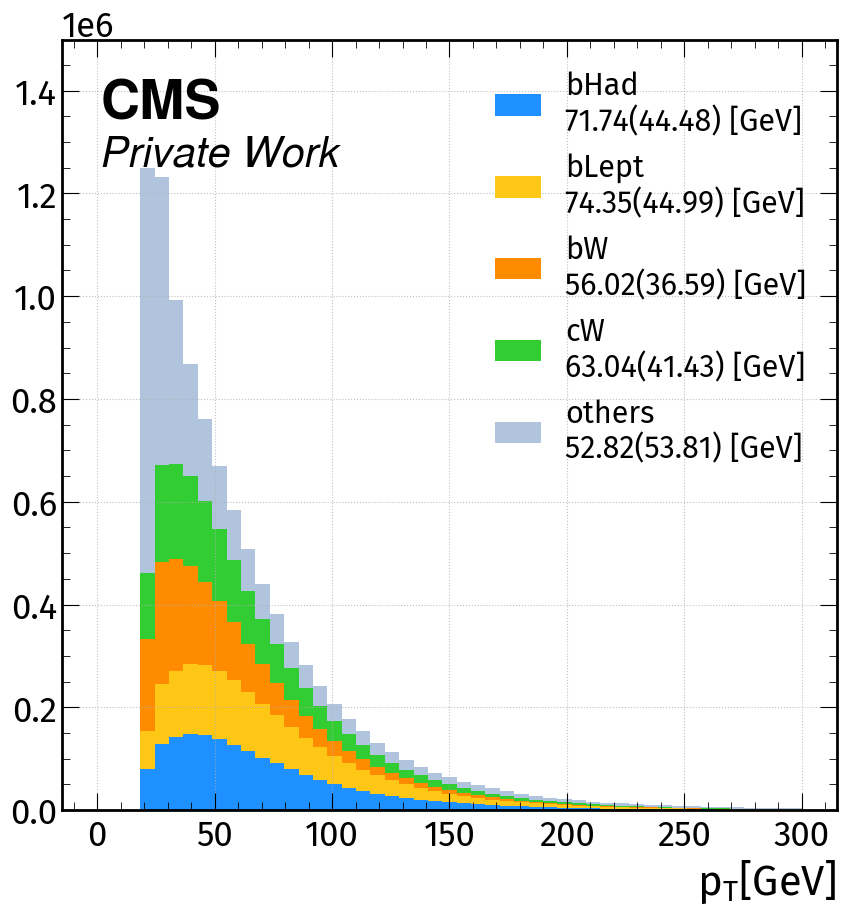
\includegraphics[width=1\linewidth]{fig//chap08-kin_reco/jets/jet_pt.png}
        \caption{Jets $p_T$}
    \end{subfigure}  
    \hfill
    
    \begin{subfigure}{0.42\linewidth}
        \hspace{0.15cm}
        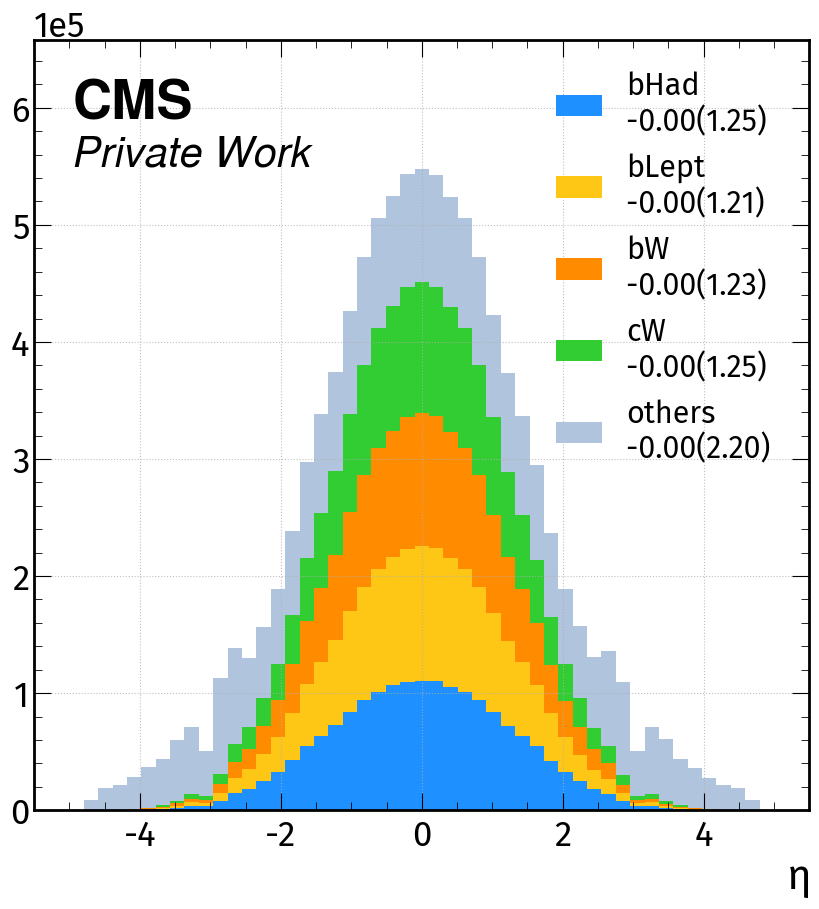
\includegraphics[width=1\linewidth]{fig//chap08-kin_reco/jets/jet_eta.png}
        \caption{Jets $\eta$}
    \end{subfigure}
    \hfill
    \begin{subfigure}{0.435\linewidth}  
        \centering
        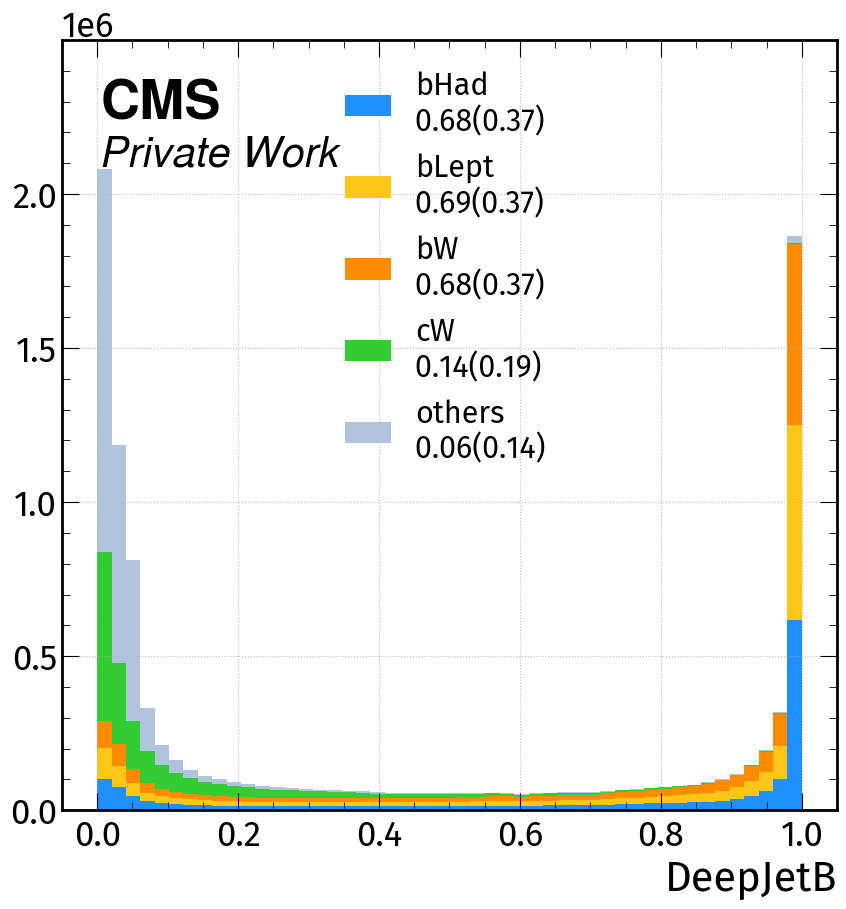
\includegraphics[width=1\linewidth]{fig//chap08-kin_reco/jets/jet_b.png}
        \caption{\DeepJet B}
    \end{subfigure} 
    \hfill
    \begin{subfigure}{0.435\linewidth}
        \centering
        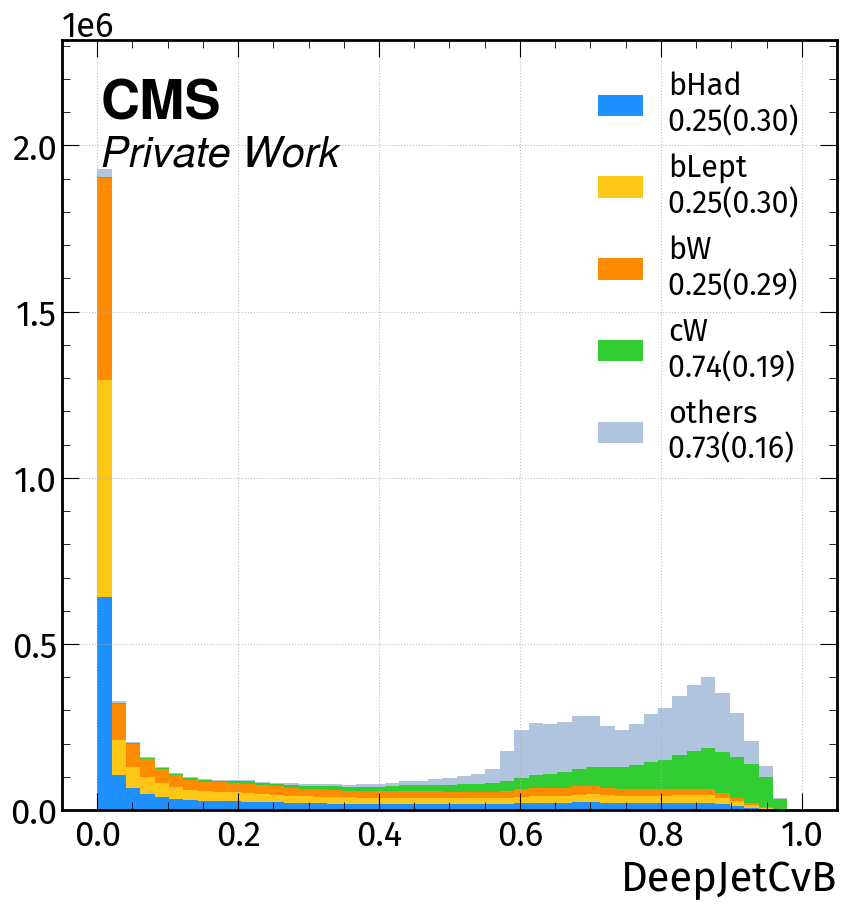
\includegraphics[width=1\linewidth]{fig//chap08-kin_reco/jets/jet_cvb.png}
        \caption{\DeepJet CvB}
    \end{subfigure}
    \hfill
    \begin{subfigure}{0.435\linewidth}  
        \centering
        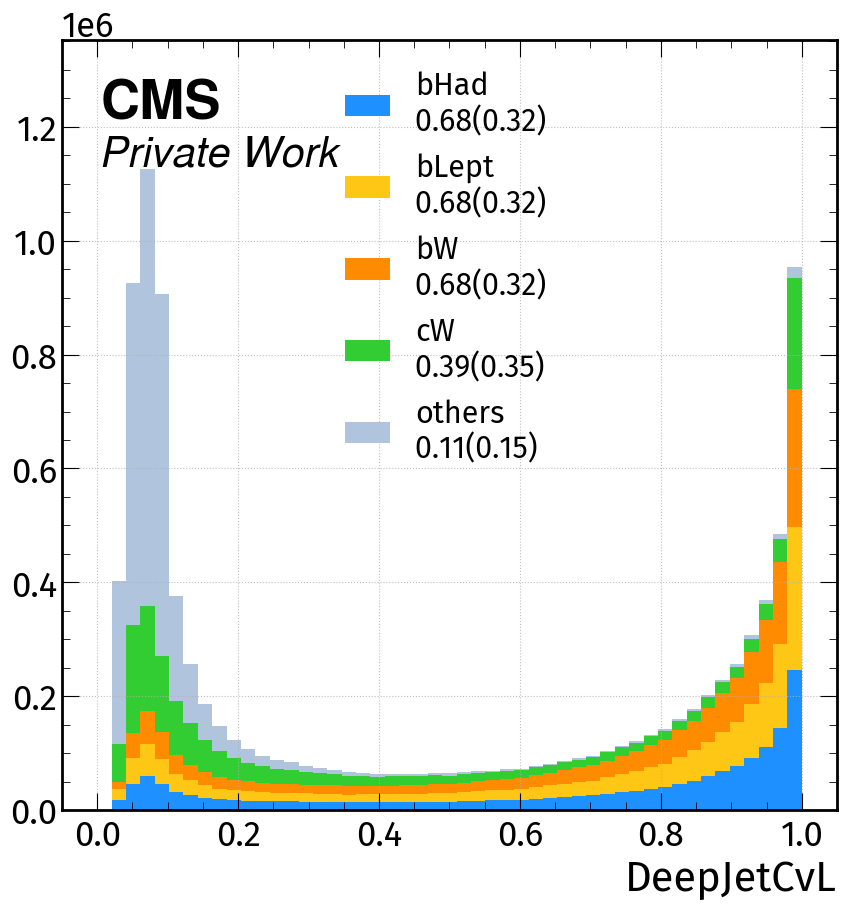
\includegraphics[width=1\linewidth]{fig//chap08-kin_reco/jets/jet_cvl.png}
        \caption{\DeepJet CvL}
    \end{subfigure}  
    \caption{Stacked plots of observables of jets that match the four quark partons.}
    \label{fig:jets_stack}
\end{figure}